% Template author: Johannes Demel
% Document class provides standardized title page + needed extras.
\documentclass{cel-thesis/cel-thesis}
\thesisTitle{Implementierung und Analyse einer DAB/DAB+ Transceiver Applikation}
\thesisType{Bachelorarbeit}
\thesisAuthor{Moritz Luca Schmid}
%\thesisAdvisor{Univ.-Prof. i. R. Dr.rer.nat. Friedrich K. Jondral}
%\thesisHeadOfInstitute{Dr.-Ing. Holger Jäkel}
\thesisSupervisor{M.Sc. Felix Wunsch}
\thesisStartDate{12.06.2017}
\thesisEndDate{05.12.2017}
\thesisSignatureDate{05.12.2017}
\thesisLanguage{ngerman} % english or ngerman
\thesisCC{FALSE}
\thesisPythonWatermark{FALSE}


%%% LANGUAGE SETTINGS %%%%%%%%%%%%%%%%%%%%%%%%%%%%%%%%%%%%%%%%%%%%%%%%%%%%%
% additional Hyphenation rules
\hyphenation{non-para-metric repro-gra-mmable}
% Settings for bibliography
\usepackage{babelbib}
\setlanguage % set correct language as selected above

%%% PACKAGES %%%%%%%%%%%%%%%%%%%%%%%%%%%%%%%%%%%%%%%%%%%%%%%%%%%%%%%%%%%%%%%%%
% Add all the packages you feel like you need them.
% You'll need it.
% automatically expand/abbreviate terms.
\usepackage{caption}
\usepackage{subcaption}
\usepackage{todonotes} % great for draft annotations
%\usepackage[latin1]{inputenc}
\usepackage{tikz}
\usepackage{mathtools}
\usepackage{amsmath}
\usepackage{amsfonts}
\usepackage{siunitx}
\usepackage{pgfplots}
\usepackage{filecontents}
\usepackage{tikz}
\usetikzlibrary{datavisualization}
\usetikzlibrary{positioning}
\usetikzlibrary{arrows,calc,fit}
\tikzset{line/.style={draw, thick, -latex'}}
\usepackage{ trfsigns}
\usepackage{tkz-euclide}
\usepackage{svg}
\usepackage{multirow}
\usepackage{float}
\usepackage{graphicx}
\usepackage{eurosym}
\usepackage{textcomp} 

%%% GLOBAL VARIABLES %%%%%%%%%%%%%%%%%%%%%%%%%%%%%%%%%%%%%%%%%%%%%%%%%%%%%%%%%%%%
\newcommand{\iterations}{200}


%%% DEFINITIONS %%%%%%%%%%%%%%%%%%%%%%%%%%%%%%%%%%%%%%%%%%%%%%%%%%%%%%%%%%%%%%%%%
%% pretty C++ print.
\def\CC{{C\nolinebreak[4]\hspace{-.05em}\raisebox{.4ex}{\tiny\textbf{++}}}}

\begin{document}
\pagenumbering{roman}  % all the preliminaries should be counted roman style
\maketitle
%% preliminaries
  \chapter*{Abstract}
This is my abstract.
CEL thesis rules require it to be about 3-5 pages. \todo{This is a todo example}
It is a summary of what you do in your thesis.
Use around 5 pictures and outline whatever you did.
And now a few lines of information.


		% a MUST, few pages abstract

%% main document
\cleardoublepage
\pagenumbering{arabic} % now old school arabic enumerated pages.
  \tableofcontents 		% a MUST
  \cleardoublepage		% make sure multipage TOCs are numbered correctly.
  \chapter{Einführung}
\label{sec:intro}
\ac{DAB} ist ein Übertragungsstandard zur Verbreitung von digitalem Radio. Das System wurde in den 90er Jahren im Zuge des Eureka 147 DAB Projekts entwickelt und kommt seit 1997 in vielen Teilen Europas und Asiens zum Einsatz. Mit dem DAB+ System, das eine Weiterentwicklung von DAB darstellt, soll langfristig die analoge \acp{UKW} Übertragung ersetzt werden.\\
Die digitale Datenübertragung bietet dabei eine verbesserte Audioqualität, da Übertragungsfehler durch Codierung empfängerseitig korrigiert werden können und somit nicht zu einem verrauschten Audiosignal wie bei FM führen. Eine Audiokompression verringert zusätzlich die Datenrate, was sich in einer gesteigerten spektralen Effizienz pro Audiokanal widerspiegelt. Die digitale Übertragung bietet außerdem viele neue Möglichkeiten der medialen Unterstützung in Form von Service Informationen wie Albumcovers, ausführlichen Stauinformationen oder Wetterkarten.\\
DAB Sender sind in sog. Ensembles strukturiert. Ein DAB Ensemble enthält ein ganzes Multiplex an Audio- und Datenkanälen. Radiosender dieses Ensembles greifen auf eine Auswahl dieser Kanäle zu. Dieses dynamische Multiplex erlaubt eine flexible und individuelle Programmgestaltung. \\
DAB stellt vier verschiedene Übertragungsmodi zur Verfügung, die für verschiedene Ausbreitungsszenarien und Frequenzbereiche ausgelegt sind. Der Fokus liegt dabei auf dem mobilen Empfang bei terrestrischer Übertragung, es existiert aber auch jeweils ein Modus für die Satellitenübertragung, sowie die niederfrequente Übetragung per Kabel. Eine Besonderheit bei DAB stellt der Einsatz von sog. Single Frequency Networks (SFNs) dar, bei denen eine Vielzahl von örtlich getrennten Sendestationen auf der gleichen Frequenz ausstrahlen. Dadurch kann ein enormer Gewinn an Frequenzeffizienz erzielt werden. Der Einsatz von SFNs wird bei DAB durch eine hohe Robustheit des Übertragungssystems gegenüber Mehrwegeempfang ermöglicht \cite{dab_buch}.\\
Ziel dieser Arbeit ist die Implementierung und Evaluation eines Senders und Empfängers für DAB/DAB+. Die Implementierung wird dabei in Form eines Software Defined Radios erfolgen, einem System bei dem ein Großteil der Signalverarbeitung auf Softwareebene durchgeführt wird. Dazu wird die Open-Source Software GNU Radio verwendet. Im Weiteren soll eine grafische Transceiver Applikation realisiert werden, die auf Basis des implementierten Senders und Empfängers eine benutzerfreundliche Oberfläche für das Senden und das Empfangen von DAB/DAB+ Signalen darstellt.

		% include chapter introduction.tex
  \chapter{DAB Standard}
\todo{Struktur mit Ensemble Services usw erklären}
\todo{Erwähnen, dass hier immer nur vom Mode 1 gesprochen wird}

Ein DAB Ensemble beinhaltet in der Regel mehrere Radio Sender und überträgt dadurch eine Vielzahl an Audio und Daten Streams im \ac{MSC}. All diese Streams werden im Main Service Multiplexer zu einem \ac{CIF} gebündelt und übertragen. Ohne Kenntnis über den Aufbau und die Struktur des Mulitplex, ist ein \ac{CIF} am Empfänger nutzlos, da keine Information über die Lage einzelner Audio Streams im Multiplex bekannt ist. Die Übertragung dieser \ac{MCI} ist Aufgabe des \ac{FIC}.

\section{FIC}
\label{sec:FIC}
Der \ac{FIC} spielt bei der Übertragung eines DAB Ensembles eine sehr wichtige Rolle, da er sowohl die \ac{MCI} als auch die \ac{SI}, wie zum Beispiel den Namen eines Radiosenders, überträgt. Die Informationen werden Paketweise in sogenannten \ac{FIG} übertragen. Die Bedeutung der \ac{MCI} wurde schon erläutert und ist naheliegend, aber auch die \ac{SI} ist von großer Bedeutung, da ein Nutzer das Radioprogramm nicht ohne dessen Namen auswählen kann. \\
Die Übertragung des FIC erfordert daher eine hohe Robustheit was durch eine gute Kanalcodierung sichergestellt wird.
%FIC chain
\begin{figure} [h]
\begin{center}
\begin{tikzpicture}
\tikzstyle{block} = [rectangle, rounded corners, draw, text width=5em, text centered, minimum height=4em]
\tikzstyle{input} = [rectangle, text width=2em, align=right, minimum height=0em]

% blocks
    \node [](null){};
    \node [input](si)[above=0.1cm of null]{SI};
    \node [input](mci)[below=0.1cm of null]{MCI};
    \node [block, right=0.8cm of null] (FIB) {FIB Quelle};
    \node [block, right=0.5cm of FIB, text width=4em] (CRC) {CRC16};
    \node [block, right=0.5cm of CRC, text width=6em] (Energy) {Energie- verwischung};
    \node [block, right=0.5cm of Energy] (conv) {Faltungs- encoder};
% arrows
    \path [line] (si.east) -- (FIB.west|-si);
    \path [line] (mci.east) -- (FIB.west|-mci);
    \path [line] (FIB.east) -- (CRC.west);
    \path [line] (CRC.east) -- (Energy.west);
    \path [line] (Energy.east) -- (conv.west);
    \path [line] (conv.east) -- ++(0.5,0);
\end{tikzpicture}
\end{center}
\label{chart:fic_encoder}
\caption{Quelle und Kanalcodierung des FIC}
\end{figure}

\subsection{\ac{CRC}}
\label{sec:crc}
Jedem \ac{FIB} der Länge 30 bytes (bestehend aus \ac{FIG}) wird ein 16 bit \ac{CRC} Wort angehängt. Das \ac{CRC} Wort wird über die 30 Nutzbytes mittels des Generatorpolynoms
\begin{equation}
G(x) = x^{16} + x^{12} + x^5 + 1
\end{equation}
berechnet. Das CRC Wort bietet keine Möglichkeit zur Fehlerkorrektur sondern dient lediglich der Fehlerdetektion, wofür es nach \cite{crc:recommendation} optimiert ist.

\subsection{Energieverwischung}
\label{sec:energieverwischung}
Im nächsten Schritt wird sichergestellt, dass die Binärquelle ideale Eigenschaften erfüllt. Dazu müssen die zu übertragenden Bits gleichverteilt sein um die Entropie der Quelle zu maximieren und zyklischen Wiederholungen von Bitsequenzen durch etwaige Wiederholungen von \ac{FIG}s müssen vermieden werden. Der Bitstream wird dazu über eine Modulo-2 Operation mit einer \ac{PRBS} gescrambled. Die \ac{PRBS} erfüllt die gewünschten Eigenschaften und ist durch das Polynom
\begin{equation}
\label{eq:energy_dispersal}
P(x) = X^9 + X^5 + 1
\end{equation}
im Empfänger exakt reproduzierbar.

\subsection{Faltungscodierung}
\label{sec:faltungscodierung}
Eine Kanalcodierung ermöglicht die Erkennung und Korrektur von Bitfehlern auf Kosten einer geringeren Nutzdatenrate. Das DAB System verwendet eine Faltungscodierung mit der Coderate $R=1/4$ und einer Einflusslänge von 7 Bits. Für jedes Eingangsbit produziert der Encoder also ein Codewort der Länge 4 bit, das über die Polynome
\begin{equation}
\begin{aligned}
g_1(x) &= 1 + x^2 + x^3 + x^5 + x^6 \\
g_2(x) &= 1 + x + x^2 + x^3 + x^6 \\
g_3(x) &= 1 + x + x^4 + x^6 \\
g_4(x) &= 1 + x^2 + x^3 + x^5 + x^6
\end{aligned}
\end{equation}
berechnet werden. \\
\todo{reinbringen, dass Blockweise? Lese Friedrichs}
Um die Coderate $R$ zu erhöhen wird die punktierte Faltungscodierung verwendet, bei der aus einer Gruppen von Codebits ein Teil der Bits wieder gestrichen (punktiert) wird. Dadurch ergeben sich eine Vielzahl an möglichen Coderaten
\begin{equation}
R_{punktiert} = \frac{8}{8 + PI} \text{mit} PI \in [1;24]
\end{equation}
wobei $R = 1/4 \leq R_{punktiert} \leq 1$ gilt.\\
Der FIC verwendet eine konstante Coderate von $R_{punktiert, FIC} = 1/3$.



\section{MSC}
% MSC chain
\begin{figure} [h]
\begin{center}
\begin{tikzpicture}
\tikzstyle{block} = [rectangle, rounded corners, draw, text width=5em, text centered, minimum height=4em]
\tikzstyle{input} = [rectangle, text width=2em, align=right, minimum height=0em]

% blocks
    % audio1
    \node [](audio1){Audio (stereo)};
    \node [](audio left)[above=0cm of audio1]{};
    \node [](audio right)[below=0cm of audio1]{};
    \node [block, right=0.4cm of audio1] (MPEG) {Audio Kompression};
    \node [block, right=0.5cm of MPEG, text width=6em] (Energy) {Energie- verwischung};
    \node [block, right=0.5cm of Energy] (conv) {Faltungs- encoder};
    \node [block, right=0.5cm of conv] (time) {Zeit- Interleaver};
    \node [right=0.5cm of time](end1){};
    % audioN
    %\node [below=1cm of audio1](audioN){\rotatebox{270}{\dotso}};
    \node [circle, draw, below of= audio1, node distance = 1.5cm](audioN){};
    \node [below of=MPEG, node distance=1.5cm](audioNpoint){};
    \node [below of=end1, node distance = 1.5cm](end2){};
    % data1
    \node [block, below of = Energy, node distance=3cm, text width=6em] (Energy2) {Energie- verwischung};
    \node [left=1cm of Energy2](data1){};
    \node [](Data text)[above=0cm of data1]{Daten};
    \node [block, right=0.5cm of Energy2] (conv2) {Faltungs- encoder};
    \node [block, right=0.5cm of conv2] (time2) {Zeit- Interleaver};
    \node [right=0.5cm of time2](end3){};
    % dataN
    \node [below of= data1, node distance = 1.5cm](dataN){rotatebox{90}{...}};
    \node [below of=end3, node distance = 1.5cm](end4){};
    % Mux
    \node (muxpoint) at ($(end1)!0.5!(end4)$) {};
    \node [rectangle, rounded corners, draw, text width=3em, text centered, minimum height=16em, right=0cm of muxpoint](mux){\rotatebox{90}{Main Service Multiplexer}};
% arrows
    % audio1
    \path [line] (audio left.east) -- (MPEG.west|-audio left);
    \path [line] (audio right.east) -- (MPEG.west|-audio right);
    \path [line] (MPEG.east) -- (Energy.west);
    \path [line] (Energy.east) -- (conv.west);
    \path [line] (conv.east) -- (time.west);
    \path [line] (time.east) -- (end1);
    % audioN
    \path [line, dotted] (audioNpoint.east) -- (end2.west);
    % data1
    \path [line] (data1.east) -- (Energy2.west);
    \path [line] (Energy2.east) -- (conv2.west);
    \path [line] (conv2.east) -- (time2.west);
    \path [line] (time2.east) -- (end3);
    % dataN
    \path [line, dotted] (dataN.east) -- (end4.west);
\end{tikzpicture}
\end{center}
\end{figure}

\todo{logical Frames, Audio und Data, Packed und Stream}
\subsection{Audio Kompression}
Die subjektiv empfundene Qualität der übertragenen Audio Streams soll der einer Audio CD gleichen. Audio CDs verwenden $16$ PCM pro Monokanal bei einer Samplerate von $44,1 kHz$. Dies entpricht einer gesamten Bitrate von $1,41 Mbit/s$ für eine einzelne Audioübertragung mit Stereokanälen. Nimmt man nun noch eine Faltungscodierung mit exemplarischer Coderate von $R=1/2$ in die Rechnung auf, übersteigt schon diese einzelne Audioübertragung die Gesamtkapazität des \ac{MSC} von $2,304 Mbit/s$ (siehe \ref{sec:MUX}). Um daher eine Vielzahl von Audiokanälen im \ac{MSC} unterbringen zu können, ist die Notwendigkeit einer Audiokompression ersichtlich, deren Kompressionsrate etwa einer Größenordnung entsprechen muss. Die verwendete Audiokompression ist \ac{MPEG 2}~\cite{etsi:mp2} für den DAB Standard und MPEG4 HE-AACv2 für DAB+. \todo{schon erklärt was DAB+ ist?! (bzw DAB+ erst nach erklärung von MPEG 2 bringen?}

\ac{MPEG 2} ist ein generischer Audiocodec der verschiedene Effekte zur verlustbehafteten Kompression verwendet. Zum einen wird die Redundanz des Audiosignals reduziert, indem durch statistische Korrelation eine Vorhersage über das Zeitsignal getroffen werden kann \cite{dab_buch}. Zudem verwendet \ac{MPEG 2} ein psychoakustisches Modell des menschlichen Ohres. Damit ist es möglich die spektrale Hörschwelle an einem bestimmten Zeitpunkt zu bestimmen. Diese Information kann genutzt werden, um das in 32 Frequenzbänder zerteilte Signal in Abhängigkeit der temporären Empfindlichkeit des Ohres zu Quantisieren und somit das Quantisierungsrauschen in jedem Frequenzband knapp unter der Hörschwelle zu halten. Abb.~\ref{chart:MPEG} zeigt dieses Prinzip als Blockschaltbild. 
\todo{Nochmal blöcke oder iwas erklären? Masking reinbringen??}
\\
% MPEG codec
\begin{figure} [h]
\begin{center}
\begin{tikzpicture}
\tikzstyle{block} = [rectangle, rounded corners, draw, text width=5em, text centered, minimum height=4em]

% blocks
    \node [](null){};
    \node [](pcm)[above=0cm of null]{PCM Audio};
    \node [block, right=1.4cm of null] (bank) {Filter- bank};
    \node [block, right=1cm of bank, text width=7em] (quantizer) {Quantisierung und Codierung};
    \node [block, right=1cm of quantizer, text width=7em] (packing) {Paketerstellung und CRC};
    \node [block, below=0.5cm of bank] (psycho) {Psycho- akustisches Modell};
    \node [block, below=0.5cm of quantizer] (alloca) {Bit Zuweisung};
    \node [right=1cm of packing](end){};
    \node [](pcm)[above=0cm of end]{MPEG 2};
% arrows
    \path [line] (null) -- (bank.west);
    \path [line] (bank.east) -- (quantizer.west);
    \path [line] (quantizer.east) -- (packing.west);
    \path [line] (psycho.east) -- (alloca.west);
    \path [line] (alloca.north) -- (quantizer.south);
    \path [line] (bank.east)++(0.5,0) |- (alloca.base west);
    \path [line] (bank.west)++(-0.5,0) |- (psycho.west);
    \path [line] (packing.east) -- (end);
    %\draw [->] (si.east) -- (FIB.west|-si);
    
\end{tikzpicture}
\caption{Blockdiagramm der MPEG 2 Kompression}
\label{chart:MPEG}
\end{center}
\end{figure}

Mit \ac{MPEG 2} lässt sich die erwähnte CD Qualität subjektiv mit einer Bitrate von etwa 192 kbit/s erreichen. Eine noch stärkere Komprimierung bietet \ac{MPEG 4}, welches nach subjektiven Hörtests dieselbe Qualität bei einer geringeren Daterate von 96 - 128 kbit/s erreich~\cite{mpeg:audio_tests}. \ac{MPEG 4} stellt eine eine Weiterentwicklung von \ac{MPEG 2} dar und basiert auf dem selben Prinzip. Um die Datenrate noch weiter zu reduzieren werden Verfahren wie Spektralbandrepilaktion und Kanalkopplung (Joint-Stereo) genutzt. Der \ac{MPEG 4} Codec wurde zusammen mit einer zusätzlichen Reed-Solomon Fehlerkorrektur in den DAB Standard integriert und wird in Deutschland seit 2011 als "DABplus\" ausgestrahlt. \todo{Spektralbandrepilkation und Kanlkopplung erklären? Mehr zu RS?}

\subsection{Energieverwischung}
Eine Energieverwischung wird wie in Abschn.~\ref{sec:energieverwischung} auch im \ac{MSC} durchgeführt.

\subsection{Faltungscodierung}
Die in Abschn.~\ref{sec:faltungscodierung} beschriebene Faltungscodierung mit anschließender Punktierung kann im \ac{MSC} genutzt werden, um die Coderate jedes einzelnen Kanals individuell einzustellen. Dabei stehen sog. Protection Level zur Verfügung die durch eine Kombination verschiedener Punktierungsmuster Coderaten von $R=1/4$ bis $4/5$ erzeugen.\\
Neben der \ac{EEP} gibt es zudem die Möglichkeit einzelne Bit-Blöcke innerhalb eines Frames stärker zu codieren als andere. Die \ac{UEP} ist zum Beispiel für MPEG Audio Frames sehr sinnvoll um die für die subjektive Audioqualität (wenigen) wichtigen Bits mit einer sehr hohen Redundanz zu versehen ohne dabei die Gesamtcoderate deutlich zu erhöhen. Ein Bitfehler im Header kann beispielsweise zu einer Fehlskalierung eines ganzen Frequenzbandes führen was sich beim Hörer als unangenehmes Pfeifen (sog. 'birdies') auswirkt, wohingegen ein einzelner Bitfehler des Zeitsignals unbemerkt bleibt.

\subsection{Zeit-Interleaving}
\label{sec:time_interleaving_std}
Die Faltungscodierung kommt schnell an ihre Grenzen, wenn anstelle von einzelnen Bitfehlern ganze Bündelfehler auftreten. Solche zeitlich begrenzten Empfangsausfälle entstehen zum Beispiel bei mobilen Empfängern in Bewegung durch Fadingeffekte. Im \ac{MSC} befindet sich mit dem Zeit-Interleaving deshalb ein zusätzliches Element in der Kanalcodierungskette, das die nicht-korrigierbaren Bündelfehler über die Zeit verteilt wodurch viele korrigierbare Einzelbitfehler entstehen. Der Zeit-Interleaver verzögert die Bits eines Frames nach den Regeln eines Interleaving Vektors um $0$ bis $15$ Logische Frames, was einer maximalen Verzögerung von $T_{delay, max} = 15 \cdot 24ms = 360 ms$ nach sich zieht. $T_{delay, max}$ entspricht also der maximalen Länge von Bündelfehlern die vom Zeit-Interleaver verteilt werden können. \todo{wirklich, oder weniger?} Gleichzeitig ist $T_{delay, max}$ aber auch die Verzögerung der Gesamtübertragung, da ein Frame erst decodiert werden kann, wenn alle Elemente (die maximal eine Verzögerung von $T_{delay, max}$ haben) empfangen wurden. Diese konstante Verzögerung wird im MSC für die verbesserte Fehlerkorrektur in Kauf genommen. Im FIC ist solch eine Verzögerung nicht möglich, da eventuell zeitkritische Daten wie zum Beispiel die Umkonfiguration des DAB Multiplexes übertragen werden, weshalb beim FIC kein Zeit-Interleaving angewendet wird.

\subsection{Multiplexing}
\label{sec:MUX}
Im Multiplexer werden alle Kanäle des MSC gebündelt. Dabei beinhaltet das resultierende \ac{CIF} jeweils ein logisches Frame aus jedem Kanal, also Daten von $24ms$ jedes Streams. Das CIF wird in sog. \ac{CU} von jeweils $64 bit$ partitioniert und besitzt eine Gesamtkapazität von $864 \ac{CU}s$, also $55296 bit$. Über die \ac{CU}s erfolgt auch die Adressierung der einzelnen Kanäle, was den wichtigsten Teil der in \ref{sec:FIC} beschriebenen \ac{MCI} ausmacht.\\
Die Kapazität des CIFs ist groß genug um eine Vielzahl von Audio- und Datenkanälen zu transportieren. \todo{Auf DAB Ensemble beziehen, das weiter oben erwähnt werden muss} Ein typischer \footnote{Bezogen auf ein in Karlsruhe (Deutschland) empfangenes DAB+ Ensembles des Südwestrundfunks.} $16 bit$ PCM Stereo Audio Stream mit der Abtastrate $32 kHz$ hat nach der Komprimierung eine Bitrate von $2\cdot64kbit/s$. Bei einem Protection Level von A3 ($\hat{=}$ Coderate $R=1/2$) können also beispielsweise 10 Audiostreams parallel übertragen werden.
Wird das CIF nicht komplett mit Kanälen gefüllt, werden die unbesetzten CUs mit einer \ac{PRBS} (siehe~\ref{sec:energieverwischung}) aufgefüllt um ein ungleiche Energieverteilung im CIF zu verhindern.

\section{OFDM Modulation}
\label{sec:ofdm_mod}
\todo{anderer Titel, sowas wie Sendesignal}


\begin{figure}
\begin{center}
\begin{tikzpicture}[inner sep=0pt]

% make a matrix to position nodes after tikz tutorial p.66
\matrix[row sep=1mm,column sep=8mm] {
% First row:
\node [](y achse oben) {}; & \\
& \\
& \\
& \\
& \\
& \\
& \\
% center start
\node [](y achse mitte) {}; &&&&&&&&& \node [](x achse rechts) {};
& \\
% center end
& \\
& \\
& \\
& \\
& \\
& \\
% Last row:
\node [](y achse unten) {}; & \\
};

% draw coordinates
\draw [-] (y achse unten) -- (y achse oben);
\draw [-] (y achse mitte) -- (x achse rechts);

%\draw [-] () -- ();

\end{tikzpicture}
\end{center}
\caption{OFDM Sendesignal}
\label{chart:transmission_frame}
\end{figure}

\subsection{Partitionierung des OFDM Frames}
\label{sec:transmission_frame}
Die Daten aus FIC und MSC werden vor der OFDM Modulation jeweils zu einem Sendeframe zusammengefasst. Ein Frame enthält dabei $4$ CIFs und deren zugehörigen FIBs, was einer Streamdauer von $4\cdot24ms = 96ms$ entspricht. Die Strukturierung des Sendeframes erfolgt in sogenannten OFDM Symbolen, die Pakete von jeweils 1536 QPSK Symbolen darstellen. $K=1536$ entspricht dabei der Anzahl der genutzten OFDM Unterträger (siehe Abschn.~\ref{sec:ofdm}). \todo{Grafik mit Frameaufteilung}
Zusätzlich zu den Datensymbolen beinhaltet jedes Frame noch das NULL Symbol und das Phasenreferenzsymbol für Synchronisationszwecke.

\subsubsection{NULL Symbol}
Das erste OFDM Symbol jedes Sendeframes $m$ ist das Nullsymbol $z_{0,k}$, für das
\begin{equation}
S(t) = 0 \; \text{für} \: t \in [0, T_{NULL}]
\end{equation}
\todo{gescheiten zeitparameter t, zumindest durchgängig gleich}
gilt. Diese Energielücke von bekannter Dauer $T_{NULL} = 1,297ms$ stellt eine Möglichkeit für eine sehr einfache und robuste grobe Zeitsynchronisation auf die Sendeframes dar.
\todo{Ansatz von dab buch mit matched filter hier oder in der implementierung??}

\subsubsection{Phasenreferenzsymbol}
\label{sec:phasenreferenzsymbol}
Das Phasenreferenzsymbol $z_{1,k}$ bildet das zweite Symbol jedes Frames. Es enthält eine vordefinierte Sequenz an komplexen \ac{CAZAC} Symbolen, deren Amplitude stets konstant, und deren Autokorrelation stets null ist. Das Phasenreferenzsymbol dient zum einen, namensgebend, als Bezugsphase für differentielle Modulation der nachfolgenden D-QPSK Datensymbole. Zum anderen eignet es sich aufgrund seiner \ac{CAZAC} Eigenschaften und der Tatsache, dass das Phasenreferenzsymbol auch im Empfänger bekannt ist, ideal für eine feine Zeitsynchronisation sowie für eine feine und grobe\footnote{Nach \cite{dab_buch} kann durch die CAZAC mittels einer AFC (Automatic Frequency Conrol) ein Frequenzoffset von $\pm 32kHz$ ($\hat{=} \pm 32 \: Unterträger$) eindeutig erkannt werden.} Frequenzsynchronisation über Korrelation.

\subsection{QPSK Modulation}
\label{sec:qpsk}
Die Bits des FIC und MSC werden mit QPSK moduliert. Dabei werden $2K=3072$ Bits ($p_{l,n}$ für $n\in[0;2K)$) zu $K=1536$ QPSK Symbolen ($q_l,n$ für $n\in[0;K)$) moduliert, wobei die erste Hälfte der Bits die Realteile $n\in [0;K)$ und die zweite Hälfte die Imaginärteile $n\in [K;2K)$ bilden, sodass sich die modulierten Symbole zu
\begin{equation}
q_{l,n} = \frac{1}{\sqrt{2}}\left[\left(1-2p_{l,n}\right)+j\left(1-2p_{l,n+K}\right)\right]
\end{equation}
ergeben.
\todo{evt. Bild mit Contellationsdiagramm}

\subsection{Frequenzinterleaving}
Die modulierten OFDM Unterträger werden vor der OFDM Modulation durch eine pseudo-zufällige Folge untereinander vertauscht. Bei langsamer Bewegung oder Stillstand führt ein Mehrwegeempfang zu langsamem selektivem Fading. Daraus resultierende Bündelfehler auf einzelnen Unterträgern übersteigen die Einflussdauer des Zeitinterleavers. Durch das Vertauschen der Unterträger werden die Effekte eines solchen frequenzselektives Fadings minimiert. \todo{samples gehen durch freq-interleaving von q zu y über}


\subsection{Differetielle Modulation}
\label{sec:diff_mod}
Die QPSK modulierten und frequenzvertauschten Unterträger werden in einem letzten Schritt vor der OFDM Modulation differentiell codiert. Die Phase jedes Sendesymbols ergibts sich aus der Summe Phase des Symbols zur Phase dessen Vorgängers.
\begin{equation}
\begin{aligned}
z_{l,k} = &z_{l-1,k}\cdot y_{l,k} = e^{j\varphi_z} \cdot e^{j\varphi_y} \\
&\text{mit} \: \varphi_z \in \{n \cdot \frac{\pi}{4}: l \: \text{gerade}\} \cup \{\frac{\pi}{4} + n \cdot \frac{\pi}{2}: l \: \text{ungerade}\}, \; n\in \mathbb{N} 
\end{aligned}
\end{equation}
Die zu übertragende Information wandert also von der eigentlichen Phase des Symbols in die relative Änderung der Phase des Vorgängersymbols zum aktuellen Symbol. Der Vorgänger des ersten Datensymbols $z_{1,k}$ eines jeden Frames ist das Phasenreferenzsymbol $z_{0,k}$ aus \ref{sec:phasenreferenzsymbol}. Die differentielle Modulation hat den großen Vorteil, dass der Empfänger den Übertragungskanal nicht kennen bzw. nicht schätzen muss. Beispielsweise habt sich eine konstante Phasendrehung im Kanal durch die Differenzbildung im Empfänger wieder auf.

\subsection{\ac{OFDM}}
\label{sec:ofdm}
Das DAB System verwendet ein \ac{FDM} zur Übertragung. Dabei werden die D-QPSK Symbole $z_{l,k}$ nicht seriell mit einer Symbolrate von $1,2 M Samples / s$ übertragen, sondern die zu übertragenden Symbole werden auf $N=2048$ Unterträgern verteilt. Die gesamte Bandbreite $B = 2,048 MHz$ wird also unter den einzelnen Unterträgern $k$ gleichmäßig aufgeteilt, sodass sich ein Unterträgerabstand von $\Delta f = \frac{B}{N} = 1kHz$ ergibt. Diese schmalbandigen und niederratigen Unterträger haben in der Summe die gleiche Symbolrate wie eine serielle Übertragung, sie bieten aber vorteilhafte Übertragungseigenschaften:
\begin{itemize}
\item Der Übertragungskanal kann pro Unterträger als flach angenommen werden.
\item \ac{ISI} wird wegen der deutlich größeren Symboldauer im Vergleich zur Seriellübertragung stark reduziert.
\end{itemize}
Das resultierende Basisbandsignal $S(t)$ ergibt sich dann als Summe der einzelnen Unterträgern, die mit dem Abstand $\Delta f$ über dem Basisband verteilt sind.

\begin{equation}
    S(t) = \frac{1}{K} \sum \limits_{k=-K/2}^{K/2} z_{l,k} \: g_{k,l}(t-lT_S) \: e^{j2\pi k \Delta f t}
\label{eq:ofdm_dft}
\end{equation}
\todo{n=0 nicht belegt wegen DC Anteil!!}

Die Symbole werden dabei mit $g_{l,k}(t)$ pulsgeformt. Damit sich die Unterträger nicht gegenseitig beeinflussen und \ac{ICI} die Performanz des Systems beschneidet, werden die Unterträger orthogonal zueinander gewählt (orthogonales \ac{FDM} (OFDM)). Das kann durch eine rechteckige Pulsformung 
\begin{equation}
\label{eq:rectangle}
\begin{aligned}
g_{k,l}(t) &= Rect(t/T_S) = 
    \begin{cases}
    1, \; \text{für} \: 0 \leq t < T_S \\
    0, \; \text{sonst}
    \end{cases}\\
\rotatebox{270}{\laplace} \\
G_{k,l}(f) &= T_S si\left(\pi f T_S\right) e^{-j \pi f T_S}
\end{aligned}
\end{equation}
erreicht werden. Wie in Abb.~\ref{fig:OFDM} zu sehen ist, haben die si-Funktionen, die sich nach \ref{eq:rectangle} aus den Rechteckfunktionen im Frequenzbereich ergeben, jeweils Nullstellen bei ganzzahligen Vielfachen von $\Delta f$, also genau an den Maxima aller anderen Unterträger. Diese Orthogonalität vermeidet \ac{ICI}, unter der Annahme dass die Unterträger an ihrer exakten Mittenfrequenz abgetastet werden.

\begin{center}
\begin{tikzpicture}
\label{fig:OFDM}
\begin{axis}[
domain=-20:20,
samples = \iterations,
height=\textwidth*0.5,
width=\textwidth,
]
    \addplot [mark=none, thick, red] {sin(deg(x))/x};
    \addplot [mark=none, densely dotted] {sin(deg(x-pi))/(x-pi)};
    \addplot [mark=none, densely dotted] {sin(deg(x+pi))/(x+pi)};
    \addplot [mark=none, dotted] {sin(deg(x-2*pi))/(x-2*pi)};
    \addplot [mark=none, dotted] {sin(deg(x+2*pi))/(x+2*pi)};
    \addplot [mark=none, dotted] {sin(deg(x-3*pi))/(x-3*pi)};
    \addplot [mark=none, dotted] {sin(deg(x+3*pi))/(x+3*pi)};
    \addplot [mark=none, very thick] {sin(deg(x))/x + sin(deg(x-pi))/(x-pi) + sin(deg(x+pi))/(x+pi) + sin(deg(x-2*pi))/(x-2*pi) + sin(deg(x+2*pi))/(x+2*pi) + sin(deg(x-3*pi))/(x-3*pi) + sin(deg(x+3*pi))/(x+3*pi)};
\end{axis}
\end{tikzpicture}
\end{center}
%\todo{article ofdm_dft zitieren und reinbringen}

Von den $N = 2048$ möglichen Unterträgern sind im DAB System nur $K = 1536$ belegt. Zum einen wurde der zentrale Unterträger ($k=0 \Leftrightarrow k\cdot \Delta f = 0kHz$) nicht belegt um einen Gleichanteil im Basisbandsignal zu vermeiden. Die restlichen unbelegten Unterträger liegen am rechten und linken Rand des Spektrums und bilden damit ein Schutzintervall gegenüber benachbarten Übertragungen.
Das gesamte Sendesignal ergibt sich letztendlich nach dem Hochmischen auf die Trägerfrequenz $f_c$ zu dem Bandpasssignal

\begin{equation}
S_{BP}(t) = \operatorname{Re} \left\{e^{j2 \pi f_c t} \sum \limits_{m=-\infty}^{\infty} \sum \limits_{l=0}^{L}   \sum \limits_{k=- \frac{K}{2}}^{\frac{K}{2}} z_{m,l,k} \: g_{k,l}(t-mT_F-T_{NULL}-(l-1)T_S) \: e^{j2\pi k \Delta f t}\right\}
\end{equation}
\todo{evt noch Guard intervall in Formle aufnehmen (t zu (t-guard time))}
Wie in \cite{ofdm:idft} gezeigt wird, kann eine \ac{IDFT} verwendet werden um das OFDM-Sendesignals zu erzeugen.
  \chapter{Implementierung eines DAB/DAB+ Transceivers}
\section{GNU Radio}
GNU Radio ist eine kostenlose und weitverbreitete Open-Source Software zur Programmierung und Ansteuerung von \ac{SDR}. Software Radio bezeichnet dabei ein Funksystem, welches die Signalverarbeitung anstatt durch Hardware (integrierte Schaltkreise) auf Softwareebene durchführt. Software hat den Vorteil, dass sie variabel und schnell austauschbar ist. Dadurch ist es möglich mit derselben Hardware viele verschiedene Funksysteme zu realisieren.\\
GNU Radio verwendet das Konzept von funktionalen Blöcken, die verbunden werden und damit eine Signalverarbeitungskette, einen sog. Flowgraph, bilden. Die einzelnen Blöcke führen jeweils eine spezifische Signalverarbeitungsoperation möglichst recheneffizient durch, weshalb ein GNU Radio Block in den meisten Fällen eine C++ Klasse darstellt. Die Ablaufsteuerung, also die Instanzierung und Anordnung der Blöcke in einem Gesamtsystem, geschieht in der Skriptsprache Python. Dazu werden die verwendeten C++ Klassen mit dem Programmierwerkzeug \ac{SWIG} nach Python übersetzt.\\
Neben der Möglichkeit, die GNU Radio Blöcke selbst zu entwerfen, gibt es schon eine umfangreiche Bibliothek an Signalverarbeitungsblöcken, die von grundlegenden Rechenoperationen bis hin zu komplexen Implementierungen wie ganzen Radarsystemen reichen. Die graphische Oberfläche \ac{GRC} ermöglicht es einen Flowgraph zu erstellen, ohne dabei Code schreiben zu müssen. Per Drag and Drop werden dazu die GNU Radio Blöcke angeordnet und mit Pfeilen verbunden. Der GRC ist ein nützliches Tool für schnelles Prototyping und für die Visualisierung eines Flowgraphs.\\

\begin{figure}[htb]
    \centering
    
\includegraphics[width=0.8\textwidth]{figures/Gnuradio_logo.png}
    \caption{Logo von GNU Radio}
    \label{fig:gnu_radio_logo}
\end{figure}

Die in diesem Kapitel vorgestellte Realisierung eines DAB/DAB+ Transceivers wurde mit GNU Radio implementiert. Das dabei enstandene Out-Of-Tree Modul gr-dab enthält alle geschriebenen GNU Radio Blöcke und Flowgraphs und ist unter der \ac{GPL3} lizenziert und frei zugänglich auf der Plattform GitHub~\cite{repo:gr-dab} veröffentlicht. Die dabei verwendete Hardware ist unabhängig von der Implemtierung und kann von kostengünstigen DVB-T Dongles bishin zu gut verarbeiteten \acp{USRP} reichen.\\
In der Evaluation des Systems in Abschn.~\ref{sec:evaluation} wurden GNU Radio Flowgraphs zudem als Basis für Simulationen genutzt.

\section{Vorgehen bei der Implementierung}
Die Implementierung des DAB/DAB+ Transceivers in GNU Radio erfolgt nach dem Bottom-up Prinzip. Einzelne Algorithmen bzw. Funktionseinheiten werden jeweils in einem C++ Block implementiert. Jeder implementierte Block wird zuerst durch einen \ac{QA} Test auf seine korrekte Funktionalität überprüft, bevor er zum Einsatz kommen kann. Oftmals hat ein Block im Sender ein entsprechendes Gegenstück im Empfänger. Es ist sinnvoll dieses Blöcke zusammen zu implementieren und gegeneinander in einem Schleifentest (Loopback) zu testen. Aus diesem Grund werden der Sender und der Empfänger synchron implementiert. Aus den einzelnen Blöcken wird anschließend eine Signalverarbeitungskette aufgebaut. Um den GNU Radio Flowgraph übersichtlich zu halten, werden verschieden Gruppen von C++ Blöcken zu sogenannten hierarchischen Blöcken zusammengefasst. Ein hierarchischer Block ist ein GNU Radio Block in Python, der mehrere C++ Blöcke intern verbindet und somit zu einem Block zusammenfasst.\\
Um größere Funktionseinheiten zu testen, werden verifizierte Referenzdaten benötigt, die aus Mangel an Alternativen über eine Antenne von einer aktiven Radiostation in der Umgebung abgegriffen werden. Damit wird zuerst der DAB Empfänger gegen die aufgenommenen Referenzdaten getestet um anschließend den Sender gegen den nun verifizierten Empfänger zu testen.\\
Im Folgenden ist aus Gründen der Übersichtlichkeit die Implementierung des Senders und Empfängers getrennt erläutert.
  \section{Implementierung des Senders}
\label{sec:imp_des_transmitters}
Abb.~\ref{fig:transmitter} zeigt den funktionsfähigen DAB Sender im GRC. Der Sender transportiert zwei Audio Kanäle im MSC, wobei der obere Kanal DAB+ (MPEG4 und Reed Solomon Encoder) und der untere Kanal DAB (MPEG 2 Encoder) transportiert. Jeder Block in der grafischen Ansicht entspricht einer eigenen C++ Klasse, wobei die Kanalcodierer des FIC und MSC, sowie der OFDM Modulator hierarchische Blöcke darstellen, also mehrere Blöcke in sich zusammenfassen. Die Struktur der Blöcke als einzelne Funktionseinheiten ist von der Aufteilung dem DAB Standard nachempfunden. Bei der Implementierung wurde darauf geachtet, möglichst viel Funktionalität in eine Klasse zu integrieren ohne dabei an Flexibilität der Blöcke einzusparen.

\begin{figure}[ht]
\centering
  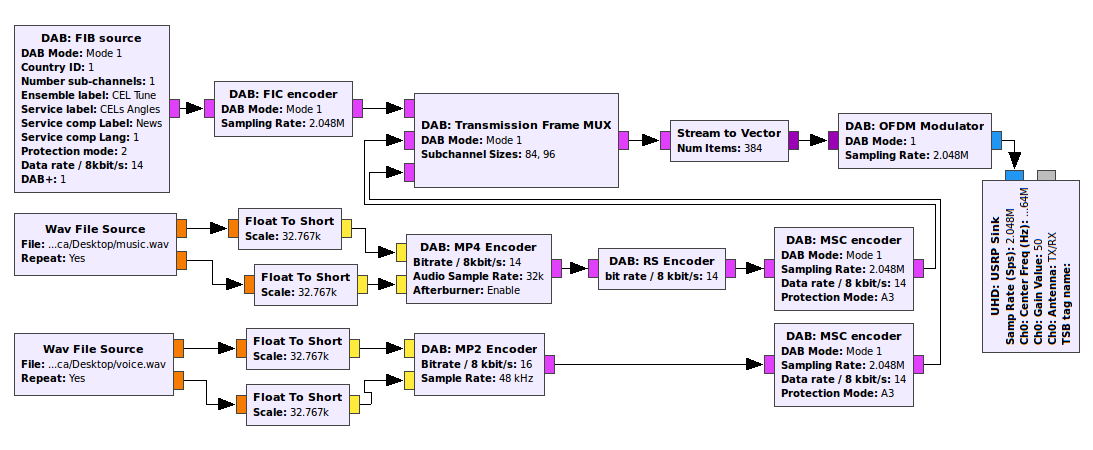
\includegraphics[width=\textwidth]{figures/GRC_transmitter.png}
	\caption{DAB/DAB+ Sender im GRC}
	\label{fig:transmitter}
\end{figure}

\subsection{FIB Quelle}
Die FIB Quelle produziert standardkonforme FIBs für den FIC. Die \ac{MCI} und \ac{SI} werden der Klasse dabei als Argumente übergeben. Die folgenden Informationen werden gesendet:
\begin{itemize}
\item Ensemble Infos: Country ID, Ensemble ID, CIF Zähler
\item Radiosender-Organisation: Country ID, Anzahl der Services, Servicebeschreibung
\item Radiosender-Komponenten: sub-channel ID, Audio Typ, primary/secondary
\item Kanal Organistaion: sub-channel ID, Start und Länge (in CUs), Protection Mode
\item Service Information (SI): Namensbeschriftung für das Ensemble und jeden Radiosender und deren Sprache
\end{itemize}
Diese FIBs umfassen bei weitem nicht das ganze Spektrum der möglichen Informationen. Sie sind aber ausreichend um dem Empfänger die nötigen MCI für die Decodierung und dem Nutzer die Informationen zur Identifikation des Programmes zur Verfügung zu stellen. Weil die MCI eine weit höhere Wichtigkeit als die SI einnimmt, wird sie mit jedem CIF geschickt. Die Größe der gesamten MCI hängt von der Anzahl der verwendeten Services und Service Komponenten ab. Bei einer Begrenzung auf maximal 7 Radiosender mit je einem Kanal kann die Information in den ersten zwei FIBs gespeichert werden. Im dritten FIB wird dann die SI gesendet.

% FIB Aufteilung
\begin{figure}[htb]
\begin{center}
\begin{tabular}{|c|c|c|c|c|}
  \hline
  \multicolumn{3}{ |c| }{\textbf{FIB 1}} & \textbf{FIB 2} & \textbf{FIB 3} \\
  \hline
  Ensemble & Radiosender & Komponente & Kanal & Service \\
  Information & Information & Information & Organisation & Information \\
  \hline
\end{tabular}
\end{center}
\caption{FIC Sendestruktur}
\label{tab:fic_struct}
\end{figure}

Da eine Namensbeschriftung mit 16 Buchstaben ein FIB schon nahezu füllt, werden die einzelnen Labels nacheinander jeweils im dritten FIB verschickt. Dies ist nicht problematisch, da die Namen der Radiosender im Regelfall über die Zeit konstant bleiben und durch eine CIF Rate von $\frac{1}{24 ms} > 41 \: \text{CIFs}/s$ trotzdem jedes Label mehrmals pro Sekunde gesendet wird.

\subsection{FIC Encoder}
\label{sec:fic_encoder}
Der FIC Encoder ist in einem hierarchischen Block implementiert, dessen beinhaltete C++ Blöcke in Abb.~\ref{fig:fic_encoder} dargestellt sind. Er enthält die gesamte Kanalcodierungskette aus Kap.~\ref{sec:FIC}. Während für die CRC Berechnung und die Faltungscodierung eine jeweilige Klasse implementiert wurde, besteht die Energieverwischung, wie in Gl.~\ref{eq:energy_dispersal} beschrieben, lediglich aus einer XOR Verknüpfung des Bitstreams mit der PRBS Folge, was mit vorhanden Blöcken realisierbar ist.

\begin{figure}[ht]
\centering
  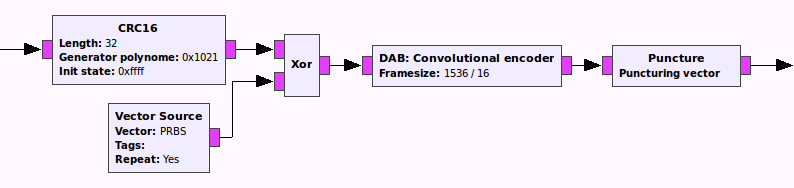
\includegraphics[width=\textwidth]{figures/FIC_encoder.png}
	\caption{Kanalcodierung im hierarchischen Block des FIC Encoders}
	\label{fig:fic_encoder}
\end{figure}

\subsection{Audio Quellen und Encoder}
Die Eingangsdaten der Audioencoder sind 16 bit \ac{PCM} Samples. Um Audio für den Stream zur Verfügung zu stellen gibt es verschiedene Möglichkeiten. Entweder werden die Audiosamples über eine Binärdatei als Rohdatenquelle genutzt. Eine andere Möglichkeit bietet der \dq WAV File Source\dq Block von GNU Radio, der aus dem populären \dq WAVE\dq Audioformat die Rohdaten extrahiert und somit auch eine PCM Quelle darstellt. Eine letzte Möglichkeit ist die direkte Generation von PCM Samples über die lokale Soundkarte. Alle drei Möglichkeiten resultieren letztendlich in einem Stream mit 16 bit Gleitkommawerten, dessen Samplingrate der Audiorate entspricht. Weil die implementierten Audiocodecs auf Integerebene arbeiten, wird der Stream vor der Encodierung auf den neuen Wertebereich abgebildet.

\subsubsection{MPEG 1/2 Audio Layer II Encoder (DAB)}
Der MPEG 2 Encoder Block verwendet einen Patch der frei verfügbare mp2 Encoder Bibliothek TooLAME. Der Patch stammt vom ODR mmbTools Projekt \cite{repo:odr_audioenc} und ist speziell auf DAB angepasst. Der Code wurde in einen GNU Radio Block integriert um ihn in einen Flowgraph einbauen zu können. Die Funktionalität des Encoder Blocks kann mit einem Loopback-Test verifiziert werden, indem der encodierte Stream mit einem Audio-Player erfolgreich und fehlerfrei decodiert und abgespielt wird.

\subsubsection{MPEG 4 HE-AACv2 (DAB+)}
Der MPEG 4 Encoder basiert auf einem Patch der FDK-AAC Codec Bibliothek für Android der Fraunhofer-Gesellschaft zur Förderung der angewandten Forschung e.V.. Die Bibliothek untersützt eine Reihe von AOTs (Audio Optimization Tools) welche die Audiokompression nach unterschiedlichen Paramtern optimieren. Es stehen die folgenden AOTs zur Verfügung:
\begin{itemize}
\item AAC-LC: Geringe Komplexität ($1,5$ bits/sample) für minimales Codierungsdelay
\item HE-AAC Dualband SBR: Hohe Effizienz ($0,625$ bits/sample) durch Spektralbandreplikation.
\item HE-AAC v2 PS: Zusätzlich mit paramterisiertem Stereo ($0,5$ bits/sample)
\end{itemize}
Ein Patch des \dq ODR-AudioEnc\dq Moduls wurde für die Implementierung des GNU Radio Blocks genutzt~\cite{repo:odr_audioenc}.\\
DAB+ enthält neben der neuen Audiokompression eine zusätzliche Fehlerkorrektur durch einen Reed-Solomon Code. Um den MPEG 4 Encoder Block nicht zu sehr auf DAB+ zu spezialisieren, wurde der Reed-Solomon Encoder in einem separaten Block implementiert.

\subsection{MSC Encoder}
Der MSC Encoder entpricht von Aufbau und Struktur dem FIC Encoder Block aus Kapitel \ref{sec:fic_encoder}. Der Block enthält eine zusätzliche Klasse für das Zeitinterleaving und besitzt keinen CRC Generator. \todo{evt mehr über Zeitinterleaving mit "history" erzählen?}

\subsection{Multiplexer}
Der Multiplexer Block hat prinzipiell die Aufgabe eines Parallel-Seriell Wandlers. Er besitzt einen Eingang für den FIC und eine variable Anzahl an Eingängen für den MSC und setzt alle Kanäle zu einem Sendesignale nach der Struktur aus Kapitel \ref{sec:transmission_frame} zusammen. Die Position der jeweiligen Audiostreams im CIF werden dabei über die selbe MCI bestimmt, die in den FIBs des FIC desselben Sendeframes stehen. Die Synchronisationssymbole $z_{0,k} \text{und} z_{1,k}$ sind an dieser Stelle noch nicht vorhanden und werden dem Sendeframe im OFDM Modulator hinzugefügt.

\subsection{OFDM Modulator}
Der OFDM Modulator Block ist ein hierarchischer Block mit vielen Unterklassen. Jede Klasse führt dabei einen der in \ref{sec:ofdm_mod} beschriebenen Schritte zur Modulation durch.

\subsubsection{QPSK Mapping}
Der QPSK Mapper bildet 1 Byte auf 4 komplexe QPSK Symbole ab. Da wie in \ref{sec:qpsk} beschrieben zuerst die Realteile und anschließend die Imaginärteile eines kompletten OFDM Symbols übertragen werden, kann der QPSK Mapper nicht Byte für Byte arbeiten, also jedes Byte direkt auf 4 QPSK Symbole abbilden. Daher arbeitet der Mapper auf Vektorbasis der Länge $1536/4$ Bits am Eingang, bzw. $1536$ Bits am Ausgang. Dies umfasst genau der Länge eines OFDM Symbols.

\subsubsection{Einfügen des Phasenreferenzsymbols}
Das Phasenreferenzsymbol wird schon als QPSK Symbol (um $\pi/4$ gedreht) generiert. Daher wird es erst nach der QPSK Modulation der Datensymbole an das Sendeframe angehängt. Das Phasenreferenzsymbol ist bei jedem Sendeframe gleich und kann deshalb im Konstruktur einmalig generiert werden.
\subsubsection{Differentielle Modulation}
Die Differentielle Modulation stellt eine einfache komplexe Multiplikation eines jeden Symbols mit dessen Vorgänger dar (siehe~\ref{sec:diff_mod}). Auch hier wird auf Vektorbasis gearbeitet.

\subsubsection{Frequenzinterleaving}

\subsubsection{\ac{IFFT}}
Die OFDM Operation kann nach~\ref{sec:ofdm} als \ac{IDFT} durchgeführt werden. Ein Teil der 2048 Unterträger sind nicht belegt. Diese müssen vor der Transformation als komplexe Nullsymbole eingefügt werden. Wegen $2048 = 2^{11}$ kann die IDFT als eine deutlich schnellere IFFT realisert werden. Ein IFFT Block ist in dem GNU Radio Modul \dq gr-fft\dq vorhanden \cite{repo:gr-fft}.

\subsubsection{Einfügen des Cyclic Prefixes}
Nach der IFFT liegt das Sendesignal nun im Zeitbereich vor. Das Einfügen des Cyclic Prefixes entspricht dem Kopieren vom Ende jedes Symbols an den Anfang. Das Einfügen eines Cyclic Prefixes ist eine weitverbreitete Technik bei OFDM. Daher existiert in GNU Radio schon ein Block mit dieser Funktionalität, der nur noch mit der passenden Symbollänge $T_S = 2048$ Samples und der Länge des Cyclic Prefixes $T_G = 504$ Samples initialisiert werden muss.

\subsubsection{Einfügen des Nullsymbols}
Als letzter Schritt in der Sendekette erfolgt das Einfügen des Nullsymbols. Dabei werden $T_{NULL}=2656$ Samples mit dem Wert $0+0j$ zwischen zwei Sendeframes geschrieben.

\subsubsection{}
Das Basisbandsignal ist nun bereit um hochgemischt und anschließend gesendet zu werden. Beide Schritte sind in dem GNU Radio Block USRP Sink vereint. Alternativ lässt sich das Basisbandsignal natürlich auch als I/Q Daten in einer Binärdatei speichern.
  \let\conjugatet\overline
\section{Implementierung des Empfängers}
\label{sec:impl_des_receivers}
Bei der Übertragung treten Störungen und Effekte auf, die das Empfangssignal vom Sendesignal abweichen lassen. Vor der Demodulation und Auswertung der Daten ist die erste Stufe des Empfängers deshalb eine Synchronisation. Ziel der Synchronisation ist das Empfangssignal so zu korrigieren, dass es dem Sendesignal wieder möglichst nahe kommt. Die anschließende Kanaldecodierung und Auswertung der Daten im FIC und MSC findet in den entsprechenden hierarchischen GNU Radio Blöcken statt. Abb.~\ref{fig:grc_receiver} zeigt den Aufbau eines DAB+ Empfängers im GRC.

\begin{figure}[h]
\centering
  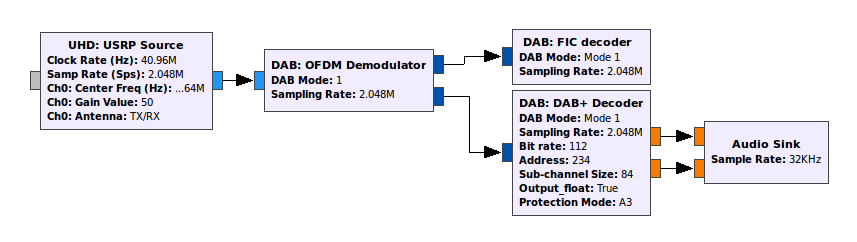
\includegraphics[width=\textwidth]{figures/GRC_receiver.png}
	\caption{DAB+ Empfänger im GRC}
	\label{fig:grc_receiver}
\end{figure}

Das Empfangssignal $R(t)$ wird in folgender Beziehung zum Sendesignal $S(t)$ angenommen:
\begin{equation}
R(t) = a(t,f) \cdot S(t-\tau_{off}) \cdot e^{j(2 \pi f_{off} t + \varphi_{off})} + N(t)
\end{equation}
Das Signal wird um einen Zeitoffset $\tau_{off}$ verzögert und hat wegen Doppler-Verschiebungen und Ungenauigkeiten der Oszillatoren einen Frequenzoffset $f_{off}$. Ein konstanter Phasenoffset $\varphi_{off}$, der durch Reflektionen der Welle entsteht, wirkt sich in diesem Fall nicht auf das demodulierte QPSK Signal aus, da sich wegen der differentiellen Modulation eine konstante Phase bei der Differenzbildung heraushebt. Es ist also keine Kanalschätzung nötig. Die Amplitude des Signals wird durch frequenzselektives Fading über der Zeit und der Frequenz unterschiedlich stark gedämpft. Wegen der Schmalbandigkeit der einzelnen Unterträger bei OFDM kann der Kanal trotzdem in jedem Unterträger als flach angenommen werden, woraus $a(t,f)=a(t)$ folgt. Die Dämpfung des Signals ist für die Symbolentscheidung bei PSK zudem nicht ausschlaggebend. Letztendlich wird das Signal noch durch \ac{AWGN} überlagert.\\ 
Um eine möglichst optimale Synchronisations zu erreichen, werden in der folgenden Signalverarbeitungskette relevanten Effekte schrittweise gemessen und korrigiert.

\subsection{Zeit Synchronisation}
\label{sec:time_sync}
Eine geeignete Zeitsynchonisation muss sowohl eine grobe Synchronisation des OFDM Frames, als auch eine feine Synchonisation der einzelnen OFDM Symbole sicherstellen. \\
Der Beginn jedes Frames $ k $ wird durch das Nullsymbol $z_{0,k}$ markiert. Wegen $S(t) = 0$ für $t \in [0, T_{\text{NULL}}]$ stellt es eine zuverlässige Möglichkeit dar, den Anfang von Frames über eine Energiemessung zu detektieren. Die Energiemessung lässt sich über eine Autokorrelation des Signals realisieren.

\begin{equation}
E[i] = \sum \limits_{j=i}^{T_G f_s + i - 1}|x[j]|^2
\label{eq:energy}
\end{equation}

Nachdem der Anfang eines Frames detektiert wurde, muss im Folgenden der Beginn jedes OFDM Symbols $z_{l,k}$ ($l \in [1, 76]$) festgelegt werden. Diese feine Zeitsynchronisation erfordert keine sehr hohe Genauigkeit, da jedem Symbol ein \ac{CP} der Dauer $T_G = 246$ \textmu s vorgeschoben ist, dessen Inhalt dem Ende des eigentlichen Symbols entspricht. Dadurch ergibt sich ein Zeitbereich von  $T_D \in [0,T_G]$, in dem der Symbolanfang fehlerfrei gesetzt werden kann. Das gesetzte Symbolfenster kann also nicht in das vorhergehende oder nachfolgende Symbol hineinragen.

\begin{figure}[htb]
\centering
  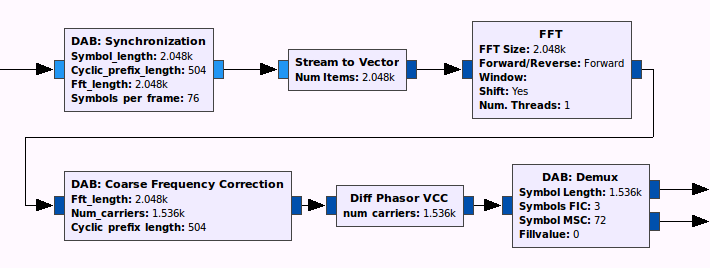
\includegraphics[width=0.9\textwidth]{figures/sync_hier_block.png}
	\caption{Aufbau der kompletten Synchronisationskette im \ac{GRC}}
	\label{fig:sync_overview}
\end{figure}

Um \ac{ISI} zu minimieren ist der theoretisch optimale Abtastzeitpunkt genau am Ende des CPs zu wählen. Eine komplette \ac{ISI} Unterdrückung ist wegen $T_G < \tau_{\text{max}}$ mit einer maximalen Echo Verzögerung von $\tau_{\text{max}} = 300$ \textmu s nicht möglich \cite{dab_buch}. Jedoch wird die \ac{ISI} zu einem Minimum reduziert, wenn ein maximal später Startpunkt gewählt wird, da die Interferenzzeit $\tau_{\text{max}} - T_D$, bei $\tau_{\text{max}} < T_G+T_S$, dadurch minimiert wird.\\

Um den exakten Anfang eines Symbols zu bestimmen, wird die zyklische Wiederholung des Symbolanteils im \ac{CP} genutzt. Durch eine Korrelation des abgetasteten Empfangssignals $r[i]$ mit einer um $T_S$ verzögerten Version desselben Signals $r[i+T_S f_s]$ über das Intervall $[i, i+T_G f_s]$ kann der Anfang des \ac{CP} über einen Peak der Korrelation identifiziert werden.

% cyclic prefix figure
\begin{figure}[h]
\begin{center}
\begin{tikzpicture}
\newcommand{\ursprung}{(0,0)}
\node[] at \ursprung (null) {}; 
\draw [thick, rounded corners = 6pt] 
    (null) -- ++(0,0.5) -- ++(0,0.5) -- ++(8,0) -- ++(0,-1) -- ++(-8,0) -- ++(0,0.5);
\draw [dashed]
    (null)+(2,0) -- ++(2,1);
\draw [dashed]
    (null)+(6,0) -- ++(6,1);
\node[] at (1,1.5) (guard) {$T_G$};
\draw [<-] (0,1.5) -- (guard.west);
\draw [->] (guard.east) -- (2,1.5);
\node[] at (5,1.5) (symbol) {$T_S$};
\draw [<-] (symbol)+(-3,0) -- (symbol.west);
\draw [->] (symbol) -- (8,1.5);
\node[] at (0.75,-0.5) (delay) {$T_D$};
\draw [<-] (delay)+(-0.75,0) -- (delay.west);
\draw [->] (delay) -- (1.5,-0.5);
%Beschriftung
\node[] at (1,0.5) (cp) {CP};
\node[] at (7,0.5) (cp) {CP Quelle};
%Vorgängersymbol
\draw [thick, rounded corners = 6pt]
    (-1.5,0) -- ++(1.5,0) -- ++(0,1) -- ++(-1, 0);
\draw [decorate,decoration={snake, amplitude=.4mm}] (-1.5,0) -- (-1,1);
%Nachfolgersymbol
\draw [thick, rounded corners = 6pt]
    (9,0) -- ++(-1,0) -- ++(0,1) -- ++(1.5, 0);
\draw [decorate,decoration={snake, amplitude=.4mm}] (9,0) -- ++(0.5,1);
%gesetztes Symbolfenster
\draw[-,decorate,decoration=brace] 
    (7.5,-0.2) -- (1.5,-0.2) node [midway, yshift=-0.3cm]{};
\node[] at (4.5,-0.6) {gesetztes Symbolfenster für $z_{l,k}$};
\end{tikzpicture}
\end{center}
\caption{OFDM Symbol und Cyclic Prefix}
\label{chart:cp}
\end{figure}

%einfache correlation
\begin{equation}
y[i] = \sum \limits_{j=i}^{T_G f_s + i - 1}r[j] r^*[j+T_S], \ \ y[i] \in \mathbb{C}
\label{eq:corr_einfach}
\end{equation}

Unter Berücksichtigung von AWGN ist $r$[i]=$x$[i]+$n$[i] mit $n[i] \sim \mathcal{N}(\mu,\,\sigma^{2})$ resultiert für die Korrelation

    \begin{alignat}{2}
y[i] &= &&\sum \limits_{j=i}^{T_G f_s + i - 1}(r[j]+n[j]) (r[j+T_S]+n[j])^* \\
&= &&\sum \limits_{j=i}^{T_G f_s + i - 1}x[j] r^*[j+T_S] + \sum \limits_{j=i}^{T_G f_s + i - 1}r[j] n^*[j+T_S] \\& &&+ \sum \limits_{j=i}^{T_G f_s + i - 1}n[j] x^*[j+T_S] + \sum \limits_{j=i}^{T_G f_s + i - 1}n[j] n^*[j+T_S] \\
&= &&\, P T_G + 2(P \sigma^2) + \sigma^4 \approx P T_G + 2(P \sigma^2)
    \end{alignat}

und damit ein SNR des Korrelationssignals von
\begin{equation}
\text{SNR} = \frac{P_s}{P_n} = \frac{P T_G f_s}{2 P \sigma^2} = \frac{T_G f_s}{2 \sigma^2}
\end{equation}

Durch eine Mittelung über $T_G f_s = 504$ Samples ist das SNR somit ausreichend groß um eine entprechend genaue Peakdetektion durchführen zu können.

Die Korrelation ist dabei auf die Energieanteile des Cyclic Prefixes und dessen Quelle nach $T_S$ normiert, sodass das Ergebnis unabhängig von der Empfangsleisung bleibt, die durch Empfangsqualität und verwendeter Hardware stark variieren kann.

\begin{equation}
    y_{\text{norm}}[i] = \frac{\sum \limits_{j=i}^{T_G f_s + i - 1}r[j] r^*[j+T_S]}{\sqrt{\sum \limits_{j=i}^{T_G f_s + i - 1}|r[j]|^2 \sum \limits_{j=i}^{T_G f_s + i - 1}|r[j+T_S]|^2}} = \frac{\sum \limits_{j=i}^{T_G f_s + i - 1}r[j] r^*[j+T_S]}{\sqrt{E[i]E[i+T_S]}}
    \label{eq:norm_corr}
\end{equation}

In Abbildung~\ref{fig:corr} ist die normierte Korrelation aus Gl.~\ref{eq:norm_corr} auf das Empfangssignal berechnet worden. Im Bereich von 1,8 bis 3,0 ms ist im Empfangssignal das Nullsymbol zu erkennen. Ein Peak der Korrelation befindet sich zum Beispiel genau bei 3 ms, was dem Ende des Nullsymbols bzw. dem Anfang des Phasenreferenzsymbols entspricht. Es ist zu erkennen, dass die Flanken der Korrelation linear ansteigen. Die Breite einer Flanke entspricht $T_G$, also gerade dem Entscheidungsbereich für $T_D$. Durch die Linearität der Flanke und der Normierung, kann der relative Abtastzeitpunkt innerhalb des CPs über einen Schwellwert eingestellt werden. Der tatsächliche Abtastzeitpunkt wird anschließend mit einer Verzögerung von $T_G$ gesetzt. In der Implementierung von Abbildung~\ref{fig:corr} wurde ein Schwellwert von $0,85$ eingestellt, der sich als guter Kompromiss zwischen \ac{ISI} Unterdrückung und einem Sicherheitsabstand zu $T_D > T_G$ herausgestellt hat. Man beachte, dass bei $T_D f_s > T_G f_s$ Samples vom nachfolgenden Symbol im gesetzten Symbolfenster lägen, was zum Empfang von falscher Information führen würde. Dieser Fall entspricht einer fehlerhaften Zeitsynchronisation.

\begin{figure}[h]
\centering
  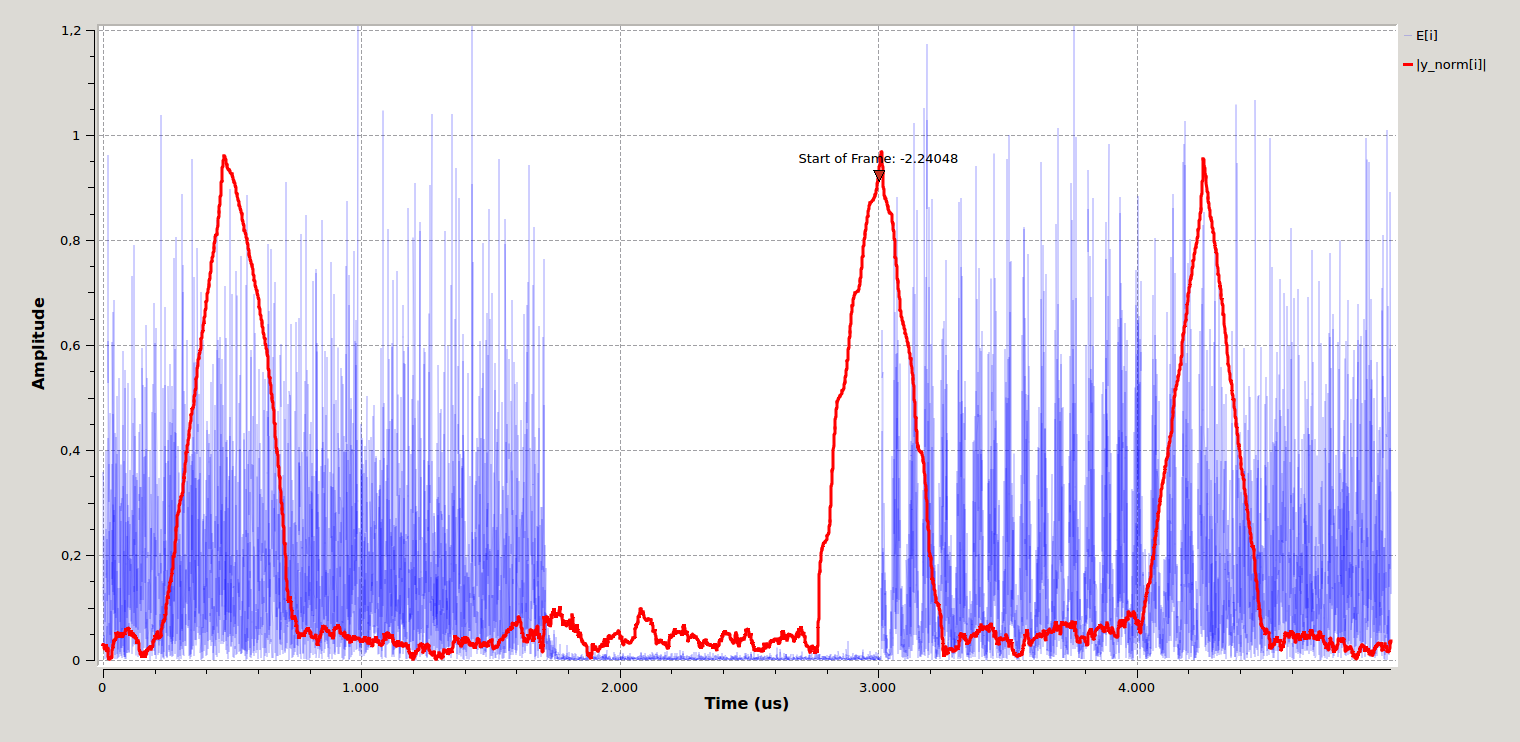
\includegraphics[width=0.8\textwidth]{figures/delayed_correlation_abs_and_energy.png}
	\caption{Korrelation des Cyclic Prefix}
	\label{fig:corr}
\end{figure}

\subsubsection{Implementierung}
Um eine mehrfache Berechnung von Gleichung~\ref{eq:energy} für die Energiemessung, sowie die normierte Korrelation (Gl.~\ref{eq:norm_corr}) zu vermeiden, wurde die feine und grobe Zeitsynchronisation in einer gemeinsamen Klasse implementiert.

\begin{figure}
\begin{center}
\begin{tikzpicture}[node distance = 2cm, auto]
% Define block styles
\tikzstyle{decision} = [diamond, draw, fill=cyan!30, 
    text width=4.5em, text badly centered, node distance=3cm, inner sep=0pt]
\tikzstyle{start} = [rectangle, draw, fill=cyan!30, 
    text width=5em, text centered, rounded corners, minimum height=4em]
\tikzstyle{class} = [rectangle, draw, dashed, 
    text width=5em, text centered, rounded corners, minimum height=4em]
\tikzstyle{output} = [trapezium, draw, fill=cyan!30, 
    text width=4em, text centered, minimum height=4em, trapezium right angle=110, trapezium left angle=70]
\tikzstyle{block} = [rectangle, draw, fill=cyan!30, 
    text width=5em, text centered, minimum height=4em]
\tikzstyle{line} = [draw, -latex']
\tikzstyle{cloud} = [draw, ellipse,fill=red!20, node distance=3cm,
    minimum height=2em]
    % Place nodes
    \node [start] (init) {Start};
    \node [decision, below of=init] (null) {NULL erwartet?};
    \node [block, below of=null, node distance=3cm] (corr) {gleitende Korrelation};
    \node [decision, below of=corr, node distance=3cm] (peak) {Peak?};
    \node [block, below of=peak, node distance=2.5cm] (energy) {Energie- messung};
    \node [decision, below of=energy] (first) {Symbol $z_{1,k}$?};
    \node [output, below of=first, node distance=3cm] (tag) {Start des Frames in $T_G$};
    \node [block, right of=null, node distance=4.8cm] (skip) {überspringe $T_S$};
    \node [block, below of=skip, node distance=3cm] (corr2) {einmalige Korrelation};
    \node [decision, below of=corr2] (peak?2) {Peak?};
    \node [above of=null, node distance=2cm] (backtonull){};
    \node [output, below of=peak?2, node distance=3cm] (lost track){nicht mehr in Sync};
    
    % klassifikation
    \node[class, minimum height=17.8cm , text width=5.5cm](search) at (0,-10.2) {};
    \node[below =0cm of search](search_text){Suche Frame Start};
    \node[class, minimum height=13.5cm , text width=3.7cm, right=0.3cm of search.north east, anchor=north west](control) {};
    \node[below =0cm of control](control_text){Kontrolle};
    
    \path [line] (init) -- (null);
    \path [line] (null) -- node {ja} (corr);
    \path [line, pos = 0.25] (null) -- node {nein} (skip);
    \path [line] (corr) -- (peak);
    \path [line] (peak) -- node {ja} (energy);
    \path [line] (energy) -- (first);
    \path [line] (first) -- node {ja} (tag);
    \path [line] (peak) -- node {nein} ++(2.5cm,0);
    \path [line] (first) -- node {nein} ++(2.5cm,0) |- (corr);
    \path [line] (skip) -- (corr2);
    \path [line] (corr2) -- (peak?2);
    \path [line] (peak?2.south) -- node {nein} (lost track);
    \path [line] (peak?2.east) -- node{ja}++(1cm,0) -- ++(0,8cm) -- ++(-6.8,0);
    \path [line] (tag) -- node{}++(0,-1cm) -- node {} ++(-2.5cm,0) -- node{}++(0,17.5cm) -- ++(2.5cm,0);
    \path [line] (lost track.south) -- ++(0,-1cm) -- ++(-2.3,0);
\end{tikzpicture}
\end{center}
\caption{Programmablaufplan der Zeitsynchronisation}
\label{chart:zeitsync}
\end{figure}

Abbildung~\ref{chart:zeitsync} zeigt den Programmablaufplan der Zeitsynchronisation. Er ist aufgeteilt in die beiden Zweige \glqq Suche Frame Start\grqq{} und \glqq Kontrolle\grqq{}. Der Zweig \glqq Suche Frame Start\grqq{} kommt bei einem der folgenden Fälle zum Einsatz:
\begin{itemize}
\item Die Synchronisation wird initial gestartet.
\item Das Programm ist nicht mehr in Synchronisation.
\item Das Ende eines Frames wurde erreicht.
\end{itemize}
Alle diese Situationen haben gemeinsam, dass im Folgenden nach dem Peak des Symbols $z_{1,k}$ (erstes Symobl nach dem Nullsymbol) gesucht wird. Dafür wird iterativ an jedem Sample des Zeitsignals $x[i]$ eine Korrelation $y[i]$ nach Gl.~\ref{eq:norm_corr} durchgeführt. Es können Korrelationspeaks, analog zu Abb.~\ref{fig:corr},  detektiert werden, die jeweils dem Start eines Symbols entsprechen. Durch die Energiemessung kann das Symbol $z_{1,k}$ von den restlichen Symbolen $z_{l,k},$ mit  $l \in [2,76]$ unterschieden werden.

Die Komplexität der Korrelationsoperation kann drastisch reduziert werden, indem die Summe, die laut Gl.~\ref{eq:corr_einfach} in jedem Schritt $T_G f_s = 504$ Additionen durchführt, durch eine gleitende Summe ersetzt wird.
%gleitende Summe
\begin{equation}
    y[i+1] = y[i] - r[i] r^*[i+T_S f_s] + r[i+T_G f_s] r^*\left[i+(T_G+T_S) f_s]\right
    \label{eq:moving_sum}
\end{equation}
Dabei ist zu beachten, dass $y[i=0]$ komplett berechnet werden muss. Die diskrete Darstellung von Gleitkommawerten im Rechner führt zu Rundungsfehlern. Aus diesem Grund wird die Summe alle $i=100000$ Samples neu berechnet, um einen Drift von $y[i]$ zu vermeiden.\\

Mit dem Anfang von $z_{1,k}$ stehen auch die Anfänge aller anderen Symbole des Frames fest, da sie mit der festen und bekannten Verzögerung von $T_G+T_S$ direkt aufeinander folgen. Der Zweig \glqq Kontrolle\grqq{} springt daher nur noch vom Start eines Symbols $x[i]$ zum nächsten $x[i+(T_G+T_S)f_s]$ und berechnet an dieser Stelle einmalig die Korrelation $y[i+(T_G+T_S)f_s]$. Liegt $y[i+(T_G+T_S)f_s]$ über einem Schwellwert, wird das Sample als Anfang des nächsten Symbols bestätigt und die Kontrollschleife iteriert zum nächsten Symbol. Falls an einem erwarteten Symbolanfang der Schwellwert der Korrelation unterschritten wird, wechselt das Programm in den Zweig \glqq Suche Frame Start\grqq{}.\\

Weil die Symboldauer genau bekannt ist, mag eine Kontrolle von jedem einzelnen Symbol zunächst überflüssig erscheinen. Der Aufwand ist jedoch gerechtfertigt, um Störeffekte wie einen Clockdrift rechtzeitig erkennen und korrigieren zu können. Ein Clockdrift kann zu einem Verlust der Synchronisation und damit zu Übertragungsfehlern führen.
Ein beispielhafter Clockdrift von 50 ppm kann im rauschfreien Fall auf dem äußersten belegten Unterträger zu einem maximalen Phasenfehler von
\begin{equation}
\begin{aligned}
    \Delta\varphi_{max} = 2 \pi f_{max} \Delta t &= 2 \pi \frac{B}{2}\, \texttt{Clockdrift}\, (T_G+T_S) \\
    &=  2 \pi \frac{1536 Hz}{2}\, 50\, \text{ppm}\; 1246\, \text{\textmu s} \\
    &= 0,3\, \text{rad} = \ang{17,2}
    \end{aligned}
    \label{eq:clockdrift}
\end{equation}
führen. Rechnung~\ref{eq:clockdrift} zeigt, dass eine feine Zeitsynchronisation zu jedem Framebeginn zu wenig ist, da sich der Phasenfehler bei 76 Symbolen pro Frame aufsummiert und damit die Entscheidungsgrenzen einer QPSK Demodulation überschreitet. Damit ist der Zweig \glqq Kontrolle\grqq{} gerechtfertigt.


%%%%%%%%%%%%%%%%%%%%%%%%%%%%%%%%%%%%%%%%%%%%%%%%%%%%%%%%%%%%%%%%%%%%%%%%%%%%%%%%%%%%%%%%%%%%%%%%%%%
\subsection{Frequenz Synchronisation}
Die Messung und Korrektur eines Frequenzoffsets $f_{off}$ ist der nächste Schritt der Synchronisationskette. Sie spielt in OFDM Systemen eine besonders wichtige Rolle, da ein Frequenzoffset die Orthogonalität zwischen den Unterträgern zerstört und zu \ac{ICI} führt.

\subsubsection{Feine Frequenz-Schätzung}
Für die Messung des Frequenzoffsets kann wieder auf die Korrelaton aus Gl.~\ref{eq:corr_einfach} zurückgegriffen werden. Ein Frequenzoffset lässt sich hier als konstante Änderung der Phase über der Zeit messen, da die Phase von \ac{CP} und dessen Wiederholung nach $T_S$ gleich sind, wenn kein Frequenzoffset vorliegt. 
\begin{equation}
f_{\text{off}}[i] = \frac{\text{arg}(y[i])}{T_S}
\label{eq:fine_frequency_estimation}
\end{equation}
Ein zusätzliches \ac{AWGN} ändert die Phase jedes einzelnen Samples. Wegen der Mittelwertfreiheit von \ac{AWGN} kann die Varianz des gemessenen Frequenzoffsets durch eine Mittelung reduziert werden.
Durch das Korrelationsintervall von $T_G f_s = 504$ Samples wird eine solche Mittelung durchgeführt, was die relativ kleine Varianz der Frequenzoffsetmessung in Abb.~\ref{plot:varianz_freq_offset} bestätigt.
\begin{figure}[htb]
\begin{center}
\begin{tikzpicture}
\begin{axis}[
xlabel={SNR [dB]},
enlarge x limits=false,
ymin=0, ymax=20,
ylabel={$E((\hat{f} - f_{off})^2) \ [Hz]$},
grid=both,
]
\addplot [blue, mark=diamond*]table {data/171020_frequency_offset_variance.dat};
\end{axis}
\end{tikzpicture}
\end{center}
\caption{Varianz der feinen Frequenzoffsetmessung}
\label{plot:varianz_freq_offset}
\end{figure}

Durch die aktive Mittelung über N Symbole wird eine weitere Senkung der Varianz um Faktor N erreicht. Pro Symbol wird genau eine Korrelation berechnet, also ergibt sich ein Mittelungsfenster der Dauer $N (T_G + T_S)$. Ein zu langes Mittelungsfenster führt zu einer Trägheit der Frequenzmessung und damit auch zu einer Zeitverzögerung in der Frequenzkorrektur, was bei schnellen Frequenzänderungen zu Synchronistaionsverlusten führen kann. Vor allem bei mobilen DAB Empfängern wird dieser Fall aufgrund der Dopplerverschiebung relevant. Deshalb wird für die obere Grenze der Mittelung die Bedingung gestellt, dass bei einer maximalen, konstanten Beschleunigung $a$ der durch die Mittelung verursachte Messfehler $f_M$ unter der $3\sigma$ Grenze der Messabweichung liegt.
\begin{equation}
f_M \overset{!}{<} \frac{3\sigma(\text{SNR})}{\sqrt{N}}
\label{eq:3sigma_grenze}
\end{equation}
Mit $a=50$ m/s$^2$ und einer Trägerfrequenz von $f_T = 200$ MHz ist
\begin{equation}
\frac{df}{dt} = f_T \frac{a}{c} = 33,3\, \text{Hz/s}
\end{equation}
und damit
\begin{equation}
\begin{aligned}
f_M &= \frac{1}{N} \sum \limits_{i=0}^{N-1}\: i \: \frac{df}{dt} (T_G+T_S) \\
&= \frac{1}{N} \frac{df}{dt} (T_G+T_S) \left(\frac{N^2 + N}{2} - N\right) \ \ {\overset{N\text{groß}}{\approx}} \ \  \frac{df}{dt} (T_G+T_S) N
\end{aligned}
\label{eq:mittelung_fehler}
\end{equation}
Aus \ref{eq:3sigma_grenze} und \ref{eq:mittelung_fehler} ergibt sich eine rauschabhängige Obergrenze für das Mittelungsintervall.
\begin{equation}
N \overset{!}{<} \left(\frac{df}{dt}\frac{T_G + T_S}{3 \sigma(SNR)}\right)^{-2/3} \overset{\text{SNR}=10\text{ dB}}{\approx} 116
\end{equation}
 %%%%%%%%%%%%%%%%%%%%%%%%%%%%%%%%%%%%%%%%%%%%%%%%%%%%%%%%%%%%%%%%%%%%%%%%%%%%%%%%%%%%%%%%%%%
\subsubsection{Grobe Frequenz-Schätzung}
Wegen arg$(y[i]) \in (-\pi,\pi]$ rad ist der gemessene Frequenzoffset aus Gl.~\ref{eq:fine_frequency_estimation} nur in $f_{off} \in (-500,500]$ Hz eindeutig. Dieser Eindeutigkeitsbereich entpricht genau der Breite eines OFDM Unterträgers von 1 kHz. Nach der feinen Frequenzkorrektur liegen also die Unterträger wieder auf dem Frequenzraster und es tritt durch die Orthogonalität keine ICI auf. Jedoch kann das Signal um das ganze Vielfache des Unterträgerabstandes verschoben sein. Das hätte zur Folge, dass Symbole im Empfänger durch eine falsche Zuweisung der FFT Bins fehlinterpretiert würden. Die Information des kompletten Frames wäre in diesem Fall verloren.\\
Da sowohl die Erkennung, als auch die Korrektur einer Unterträgerverschiebung im Frequenzbereich wesentlich einfacher ist, wird die grobe Frequenz-Korrektur nach der FFT Operation (Abschn.~\ref{sec:FFT}) durchgeführt.
Von den 2048 Unterträgern, welche aus der FFT resultieren, sind jeweils die ersten $K = \frac{1536}{2}$ rechts und links des zentralen DC-Trägers belegt. Die restlichen unbelegten Träger enthalten am Empfänger bei vernachlässigter \ac{ICI} lediglich \ac{AWGN}. Durch eine Korrelation des FFT Vektors mit dem Vektor der bekannten Trägerbelegung $[1,1,...,1,0,1,...,1,1]$ der Länge $1536+1$ kann der Trägeroffset n und der erste belegte Unterträger $X[n]$ ermittelt werden.
\begin{equation}
n = \argmax_i \sum \limits_{j=i}^{i+K-1} |X[j]|^2 \ \ \text{mit} \ \ i \in [0,L_{FFT}-K)
\end{equation}

\subsection{FFT}
\label{sec:FFT}
Die modulierten Symbole werden durch das OFDM System parallel auf den $K=1536$ Unterträgern moduliert und sind innerhalb eines Sendesymbols $T_S$ durch ihre Phase und Frequenz vollständig beschrieben \cite{nt1}. Um aus dem empfangenen Zeitsignal nach der Zeit- und Frequenzsynchronisation nun die D-QPSK Symbole zu erhalten, wechselt man mittels einer \ac{DFT} in den Frequenzbereich, was in Gl.~\ref{eq:ofdm_dft} gezeigt wurde. Wegen $L_{DFT} = \frac{2,048 \text{ M samples/s}}{T_S} = 2048 = 2^{11}$ kann die \ac{DFT} durch eine \ac{FFT} der Länge 2048 effizient implementiert werden \cite{fft:sus}. Der \ac{FFT} Algorithmus ist in GNU Radio \cite{repo:gr-fft} bereits implementiert und wird verwendet.

\subsection{Frequenzspreizung}
Die im Sender vorgenommene Frequenzspreizung wird rückgängig gemacht, indem die Unterträger wieder in ihre ursprüngliche Reihenfolge gebracht werden. Diese Operation entpricht, genau wie im Sender, einem Vertauschen der Unterträger nach einer festgelegten Vertauschungsregel. Deshalb kann hier die gleiche Klasse wie im Sender genutzt werden, die mit dem invertierten Vertauschungsvektor initialisiert wird.

\subsection{Demodulation}
Die differentielle Demodulation erfolgt durch eine komplexe Multiplikation des D-QPSK Symbols mit dessen komplex konjugierten Vorgängersymbols.\\
An dieser Stelle würde entsprechend der Umkehrung des Senders nun die QPSK Demodulation erfolgen, indem eine Bitentscheidung der komplexen Eingangswerte zum Beispiel nach dem \ac{ML}-Kriterium erfolgt. In dieser Implementierung wird aber an dieser Stelle noch keine sog. Harddecision durchgeführt. Stattdessen werden die verrauschten QPSK Symbole in ihren Real- und Imaginärteil zerlegt und als Gleitkommawerte, sog. Softbits, weitertransportiert. Eine Bitentscheidung wird in der Faltungsdecodierung über den Viterbialgorithmus mit euklidischem Abstand getroffen.

\subsection{Kanaldecodierung}
Die Kanaldecodierung durchläuft die Encodierungskette in umgekehrter Reihenfolge und stellt so schrittweise den gesendeten Bitstream wieder her.

\subsubsection{Zeitinterleaving}
Das Zeitinterleaving hat im Sender die Bits nach festen Regeln mit einer Verzögerung versehen. Der Bitstream kann also wiederhergestellt werden, indem dieselbe Verzögerung angewendet wird, um mit dem Schreiben auf das jeweilige Bit zu warten. Damit ein komplettes Symbol geschrieben werden kann, benötigt der Interleaverblock neben dem aktuellen Symbol auch alle 15 nachfolgenden Symbole. Der Block benötigt also ein Gedächtnis von 15 Symbolen. Die in \ref{sec:time_interleaving_std} angesprochene Verzögerung äußert sich in diesem Fall darin, dass die ersten 15 produzierten Symbole des Blocks kein ausreichend großes Gedächtnis haben und die entstandenen Symbole daher fehlerbehaftet sind. Wegen der Fehlerkorrekturfähigkeit des im folgenden Abschnitts beschriebenen Faltungsdecoders ist es aber praktisch sogar möglich, die tatsächliche Verzögerung um einige Symbole zu reduzieren, da die letzten verzögerten Bits vom Decoder schon a priori bestimmt werden können.

\subsubsection{Faltungsdecodierung und Viterbi-Algorithmus}
Der Faltungsdecoder nutzt die im Encoder eingefügte Redundanz, um aus der empfangenen Bitfolge die wahrscheinlichste Sendefolge zu bestimmen. Das \ac{MAP} Kriterium ist wegen der Gleichverteilung der Sendesymbole gleich dem \ac{ML} Kriterium. Um die Komplexität des Entscheiders von exponentieller Ordnung auf lineare Ordnung zu reduzieren, wird der Viterbi-Algorithmus zur Entscheidungsfindung herangezogen \cite{nt1}. Eine effiziente Implementierung eines Softbit QPSK Viterbi Decodierers ist im GNU Radio Modul \textit{gr-trellis} vorhanden \cite{repo:gr-trellis}.

\subsubsection{Scrambling}
Die angewendete Energieverwischung kann rückgängig gemacht werden, indem die selbe Operation wie im Empfänger angewendet wird. Die identischen Bits $y[i]$ der \ac{PRBS} löschen sich zu jedem Sample $i \in \mathbb{N}$ durch die Exklusiv-Oder Verküpfung gegenseitig aus, sodass wieder das Sendebit $x[i]$ entsteht.
\begin{equation}
    x[i] \oplus y[i] \oplus y[i] = x[i], \; \; \; x[i],y[i] \in \{0,1\}
\end{equation}
Die Bits haben nun die Kanaldecodierungskette durchlaufen und entsprechen im besten Fall den FIBs im FIC bzw. den komprimierten Audiostreams im MSC.

\subsection{FIC Senke}
Bevor die Informationen aus den FIBs verarbeitet werden, wird ein \ac{CRC} durchgeführt. Dazu wird aus den Datenbits wie in \ref{sec:crc} das CRC Wort berechnet und dieses mit dem gesendeten CRC Wort verglichen. Stimmen die beiden Wörter überein, enthält der FIB mit hoher Wahrscheinlichkeit keine Bitfehler. Korrekt übertragene FIBs können dann im Folgenden gelesen und ausgewertet werden.

\subsection{Audio Decoder}
Die Audiodecoder haben die Aufgabe aus dem Bitstream wieder ein PCM Stream zu generieren, der dem ursprünglichen Audiostream vor der Kompression möglichst nahe\footnote{Im Sinne einer subjektiven Wahrnehmung des menschlichen Gehörs.} kommt.
\subsubsection{DAB}
Für die Implementierung des MPEG-1/2 Audio Layer II Decoders für DAB wird die Bibliothek \textit{kjmp2} \cite{repo:kjmp} genutzt. Die Decoder werden jeweils in einen GNU Radio Block implementiert.\\
\subsubsection{DAB+}
Der Decoder für DAB+ Audio Frames wird in 3 separate Klassen implementiert, die neben der eigentlichen MPEG 4 Decodierung zusätzlich die für den DAB+ Standard eingeführte Fehlerkorrektur realisieren. Abb.~\ref{fig:dab+chain} zeigt den Signalfluss im DAB+ Audio Decoder.\\
Die erste Klasse beinhaltet den Firecode-Checker, der einen CRC durchführt um Bitfehler im Header des DAB+ Superframes zu identifizieren. In dieser Implementierung hat der Firecode-Checker zusätzlich die Funktion, den Stream auf die DAB+ Superframes zu synchronisieren. Die Synchronisation ist notwendig, weil ein DAB+ Superframe aus 5 Logischen Frames besteht, welche nacheinander über den physikalische DAB/DAB+ Kanal übertragen werden. Vor der MPEG4 Decodierung müssen daher 5 Logische Frames zu einem Superframe gepackt werden, was bei einem fortlaufendem Stream und willkürlichem Betrachtungsfenster nicht eindeutig definiert ist.\\
Die Synchronisation wird in dieser Implementierung ohne technischen Mehraufwand realisiert, indem bei nicht-erfolgreichem Firecode-Check anstelle eines ganzen Superframes nur ein Logisches Frame verworfen wird. Im nicht-synchronisierten Fall geht der Firecode-Checker somit alle Logischen Frames nacheinander durch, bis er schließlich, im bitfehlerfreien Fall, nach maximal 4 verworfenen Logischen Frames den Anfang des nächsten Superframes durch einen erfolgreichen Firecode-Check identifiziert hat.\\

\begin{figure}[htb]
\begin{center}
\begin{tikzpicture}[node distance = 1cm, auto]
\tikzstyle{block} = [rectangle, rounded corners, draw, text width=6em, text centered, minimum height=1.3cm]
\tikzstyle{Text} = [rectangle, rounded corners, text width=6em, text centered, minimum height=1.3cm]
\tikzstyle{rect} = [rectangle, draw, text width=9em, text centered, minimum height=2em]
\tikzstyle{input} = [rectangle, text width=2em, align=right, minimum height=3cm]

\node [block, text width=1.8cm](fire){Firecode Checker};
\node [Text, left=0.5cm of fire, text width=1.3cm, anchor=east](log){Logische Frames};
\node [block, right=1.2cm of fire, text width=2.5cm](rs){Reed-Solomon Decoder};
\node [block, right=1.2cm of rs, text width=2.8cm](mp4){MPEG 4 HE-AACv2 Decoder};
\node [Text, right=0.5cm of mp4, text width=2.1cm](super){DAB+ Superframes};
\node [Text, below=1cm of rs.south west, text width=3.5cm](n1){Logische Frames mit fehlgeschlagenem Firecode-Check};
\node [Text, below=1cm of mp4.south west, text width=3.3cm](n2){Nicht korrigierbare Superframes};

\path [line] (fire.10) -- (rs.170|-fire.10);
\path [line] (rs.10) -- (mp4.170|-rs.10);
\path [line] (mp4) -- (super);
\draw [line] (fire.350) to [bend left=35] (n1);
\draw [line] (rs.350) to [bend left=35] (n2);
\draw [line] (log) -- (fire);

\end{tikzpicture}
\end{center}
\caption{DAB+ Audio Decoder}
\label{fig:dab+chain}
\end{figure}

Der nachgeschaltete Reed-Solomon Decoder wurde auf Basis der Bibliothek für Vorwärtsfehlerkorrektur \textit{libfec} implementiert \cite{repo:kjmp}. Ein Superframe wird über die eingefügten Codewörter auf Blockbasis korrigiert. Nicht korrigierbare Blöcke werden verworfen.\\
Alle Superframes, die den Firecode-Checker sowie den Reed-Solomon Decoder durchlaufen haben, sind mit hoher Sicherheit korrekt und können schließlich vom Audiodecoder verarbeitet werden. Für den eigentlichen MPEG 4 HE-AACv2 wurde eine Minimal-Implementation von \cite{etsi:mp4} des Open-Source Projekts \textit{qt-dab} genutzt \cite{repo:qt-dab}.
  \chapter{Implementierung einer grafischen Transceiver Applikation}
  \chapter{Evaluation des Systems}

\begin{center}
\begin{tikzpicture}
\begin{axis}[
title=\ac{FIB} Fehlerrate,
ymode=log,
xlabel={$SNR \ [dB]$},
ylabel={FIB Fehlerrate},
grid=major,
]
\addplot [blue, mark=diamond*]table {data/171022_fic_error_rate.dat};
\addplot [red, mark=diamond*]table {data/171022_fic_throughput_rate.dat};
\end{axis}
\label{plot:varianz_freq_offset}
\end{tikzpicture}
\end{center}

\begin{center}
\begin{tikzpicture}
\begin{axis}[
title=BER,
ymode=log,
xlabel={$SNR \ [dB]$},
ylabel={BER},
grid=major,
]
\addplot [blue, mark=diamond*]table {data/171026_BER.dat};
\end{axis}
\label{plot:varianz_freq_offset}
\end{tikzpicture}
\end{center}
  %\acresetall
% This is an example chapter from 'Polar Codes for Software Radio'. Do not use it but delete it! It serves as an example!
\chapter{System model}\label{chapter:systemmodel}
Polar codes are defined for a specific system model.
The objective of this chapter is to introduce the key concepts.
Notations are introduced and important terms are revisited in order to refer to them.

\section{Key channel coding concepts}
The system model used throughout this thesis follows the remarks in \cite{Richardson:2008:MCT} and \cite{polar:arikan09}.
It is intended to define the domain for which polar codes are developed.

The objective of channel coding is to transmit information from a source to a sink over a point-to-point connection with as few errors as possible.
A source wants to transmit binary data  $u \in \mathcal{U} = \{0, 1\}$ to a sink where $u$ represents one draw of a binary uniformly distributed random variable.
The source symbols are encoded, transmitted over a channel and decoded afterwards in order to pass an estimate $\hat{u}$ to a sink.

This thesis uses a common notation for vectors which is introduced here shortly.
A variable $x$ may assume any value in an alphabet $x \in \mathcal{X}$.
Multiple variables are combined into a vector $x^N = (x_0, \dots , x_{N-1})$ of size $N$ with its alphabet $x^N \in \mathcal{X}^N$.
A subvector of $x^N$ is denoted $x_i^j = (x_i, \dots, x_{j-1})$ where $0 \leq i \leq j \leq N$.
A vector where $i=j$ is an empty vector.
A vector $x^N$ may be split into even and odd subvectors which are denoted $x_{0,e}^{2n} = (x_0, x_2, \dots, x_{2n-2})$, $x_{0,o}^{2n} = (x_1, x_3, \dots, x_{2n-1})$.
This numbering convention is in accordance with \cite{dijkstra:zerocounting}, where the author makes a strong point for this exact notation and some papers on polar codes follow it too, e.g. \cite{polar:talvardy:howtoCC}.


\subsection{Encoder}
The encoder takes a frame $u^k$ and maps it to a binary codeword $x^N$, where $k$ and $N$ denote the vector sizes of a frame and a codeword respectively with $k \leq N$.
An ensemble of all valid codewords for an encoder is a code $\mathcal{C}$.
It should be noted that $|\mathcal{C}| = |\mathcal{X}^N|$ must hold in order for the code to be able to represent every possible frame.

Not all possible symbols from $\mathcal{X}^N$ are used for transmission.
The difference between all possible codewords $2^N$ and used codewords $2^k$ is called redundancy.
With those two values, the code rate is defined as $R = \frac{k}{N}$.
It is a measure of efficient channel usage.

The encoder is assumed to be linear and to perform a one-to-one mapping of frames to codewords.
A code is linear if $\alpha x + \alpha' x' \in \mathcal{C}$ for $\forall x, x' \in \mathcal{C}$ and $\forall \alpha, \alpha' \in \mathbb{F}$ hold.
It should be noted that all operations are done over the Galois field GF(2) or $\mathbb{F} = \{0, 1\}$ if not stated otherwise.
Then the expression can be simplified to 
\begin{equation}
 x + x' \in \mathcal{C} \quad \textrm{for} \quad \forall x, x' \in \mathcal{C}.
\end{equation}
A linear combination of two codewords must yield a codeword again.

For linear codes it is possible to find a generator matrix $G \in \mathbb{F}^{k \times N}$ and obtain a codeword from a frame with $x^N = u^k G^{k \times N}$.
All linear codes can be transformed into systematic form $G = I_k P$.
$I_k$ is a $k \times k$ dimensional identity matrix.
If $G$ is systematic, all elements of a frame $u^k$ are also elements of the codeword $x^N$.
Also, a parity check matrix $H = -P^T I_{N-k}$ with dimensions $(N-k) \times N$ can be calculated from $G$.
A parity check matrix satisfies $\forall x \in \mathcal{C}: H x^T = 0^T $.
Thus, a parity check matrix can be used to verify correct codeword reception and furthermore error correction may be performed.
Error correction with $H$ may be done, e.g. syndrome decoding.

A code can be characterized by the minimum distance between any two codewords.
In order to obtain this value we use the Hamming distance.
This distance $d(v^N,x^N)$ equals the number of positions in $v^N$ that differ from $x^N$.
Minimum distance of a code is than defined by $d(\mathcal{C}) = \min\{d(x,v): x,v \in \mathcal{C}, x \neq v\}$.
For linear codes this can be simplified to comparing all codewords to the zero codeword $d(\mathcal{C}) = \min\{d(x,0): x \in \mathcal{C}, x \neq 0\}$ which is called Hamming weight.

\subsection{Channel model}\label{sec:channel_model}
Channel coding relies on a generic channel model.
Its input is $x \in \mathcal{X}$ and its distorted output is $y \in \mathcal{Y}$.
A channel is denoted $W: \mathcal{X} \rightarrow \mathcal{Y}$ along with its transition probability $W(y|x), x \in \mathcal{X}, y \in \mathcal{Y}$.
A \ac{DMC} does not have memory, thus every symbol transmission is independent from any other.
Combined with a binary input alphabet it is called a \ac{BDMC}.
For a symmetric channel model, $P(y|1) = P(-y|-1)$ must hold for an output alphabet $y \in \mathcal{Y}, \mathcal{Y} \subset \mathbb{R}$ \cite{Richardson:2008:MCT}.
Assuming symmetry for a \ac{BDMC} leads to a symmetric \ac{BDMC}.
In Sec. \ref{theory:channels} several examples of such channels are discussed.

This channel concept may be extended to vector channels.
A vector channel $W^N$ corresponds to $N$ independent uses of a channel $W$ which is denoted as $W^N : \mathcal{X}^N \rightarrow \mathcal{Y}^N$.
Also, vector transition probabilities are denoted $W^N(y^N|x^N) = \prod_{i=0}^{N-1} W(y_i|x_i)$.

\subsection{Decoder}
A decoder receives a possibly erroneous codeword $y$ and checks its validity by asserting $H y^T = 0^T$, thus performing error detection.
A more sophisticated decoder tries to correct errors by using redundant information transmitted in a codeword.
An optimal decoder strategy is to maximize the a-posteriori probability.
Given the probability of each codeword $P(x)$ and the channel transition probability $P(y|x)$, the task at hand is to find the most likely transmitted codeword $x$ under the observation $y$, $P(x|y)$.
This is denoted
\begin{equation}
 \hat{x}^{MAP} = \argmax_{x \in \mathcal{C}} p(x|y) = \argmax_{x \in \mathcal{C}} p(y|x) \frac{p(x)}{p(y)} = \argmax_{x \in \mathcal{C}} p(y|x) p(x)
\end{equation}
with Bayes' rule.
Assume every codeword is transmitted with same probability $P(x^{(i)}) = P(x^{(j)}), \; \forall x^{(i)}, x^{(j)} \in \mathcal{C}$.
This simplifies the equation and yields a \ac{ML} decoder
\begin{equation}
 \hat{x} = \argmax_{x \in \mathcal{C}} p(y|x)
\end{equation}
which estimates the most likely codeword to be transmitted given a received possibly erroneous codeword \cite{Richardson:2008:MCT}.
This decoding principle could be employed in conjunction with the Hamming distance and thus yield $\hat{x} = \argmin_{x \in \mathcal{C}} d(x, y)$.
In conclusion the task at hand is to find a code which inserts redundancy intelligently, so a decoder can use this information to detect and correct transmission errors.

\subsection{Asymptotically good codes}\label{theory:repetition_code}
A repetition code is a very simple code which helps clarify certain key concepts in the channel coding domain.
Assume the encoder and decoder use a repetition code.
For example a repetition code with $k=1$ and $N = 3$ has two codewords $\mathcal{C} = \{000, 111\}$.
Thus in this example $R=\frac{1}{3}$.
We can also obtain its generator and parity check matrices.
\begin{equation}
 G = \begin{pmatrix} 1 & 1 & 1 \end{pmatrix},\qquad H = \begin{pmatrix} 1 & 1 & 0 \\ 1 & 0 & 1 \end{pmatrix}
\end{equation}
$H$ can be used to detect if a transmission error occurred by verifying if $H x^T = 0^T$.
In case an error occurred, a \ac{ML} decoder does a majority decision to estimate the most likely codeword.

Repetition codes shed light on a problem common to a lot of codes.
If reliability of a code needs to be improved, it comes at the expense of a lower code rate.
Increasing $N$ comes at the expense of decreasing $R = \frac{1}{N}$ because $k=1$ for all repetition codes.
Thus for a very reliable repetition code $\lim_{N \rightarrow \infty} R$ tends towards $0$.

The above results leads to the definition of asymptotically good codes $\mathcal{C}(N_s, k_s, d_s)$ \cite{Friedrichs:2010:error-control-coding}.
Two properties must hold for this class of codes,
\begin{equation}
 R = \lim_{s \rightarrow \infty} \frac{k_s}{N_s} > 0 \quad \textrm{and} \quad  \lim_{s \rightarrow \infty} \frac{d_s}{N_s} > 0.
\end{equation}
The code rate must be $>0$ for all codes which repetition codes do not satisfy.
And the distance between codewords must grow proportionally to the code block size.

\section{Channels}\label{theory:channels}
Several common channel models exist to describe the characteristics of a physical transmission.
Common properties were discussed in Section \ref{sec:channel_model} whereas in this Section the differences are targeted.
The three most important channel models for polar codes are presented, namely the \ac{BSC}, the \ac{BEC} and the \ac{AWGN} channel.

\subsection{AWGN channel}
An \ac{AWGN} channel as used in this thesis has a binary input alphabet and a continuous output alphabet $\mathcal{Y} = \mathbb{R}$.
Each input symbol is affected by Gaussian noise to derive an output symbol.
Its average corresponds to the input symbol value and the variance can be interpreted as a measure of noise.
Often the input is \ac{NRZ} encoded which turns a \ac{ML} decision for a symbol into a sign decision.

\subsection{Capacity and reliability}
Channels are often characterized by two important measures, capacity and reliability.
These measures are introduced in this Section.
Channel capacity for symmetric \ac{BDMC} can be calculated by
\begin{equation}
 I(W) = \frac{1}{2} \sum_{y \in \mathcal{Y}} \sum_{x \in \mathcal{X}} W(y|x) \log_2 \frac{W(y|x)}{\frac{1}{2} (W(y|0) + W(y|1))}.
\end{equation}
It defines the highest rate at which a reliable transmission over a channel $W$ can be conducted while the error probability may still tend towards $0$.
It is also called the Shannon capacity \cite{sha49} for symmetric channels.
The Bhattacharyya parameter
\begin{equation}
 Z(W) = \sum_{y \in \mathcal{Y}} \sqrt{W(y|0) W(y|1)}
\end{equation}
is used to quantify a channel's reliability where a lower value for $Z(W)$ indicates higher reliability.
It is also referred to as Z-parameter for obvious reasons.
Also, an upper \ac{ML} decision error bound is given by $Z(W)$ \cite{polar:arikan09}.
		% an example chapter
  \chapter{Conclusion}\label{chapter:conclusion}
So you made it!
This is the last part of your thesis.
Tell everyone what happened.
You did something... and you could show that ... followed.

In the end make a personal statement.
Why would one consider this thesis to be useful?


		% everything ends with a summary!


%% Appendix
\appendix
%  \listoffigures		% if you want, not usual
%  \listoftables		% if you want, not usual
  % This file provides Abbreviations
% Sorting them is a good idea because the acronym package won't!
\chapter{Abkürzungsverzeichnis}
\begin{acronym}[TROLL]
  \acro{AGC}[AGC]{Automatic Gain Control}
  \acro{AKF}[AKF]{Autokorrelationsfunktion}
  \acro{API}[API]{Application Program Interface}
  \acro{AWGN}[AWGN]{Additives Weißes Gaußsches Rauschen}
  \acro{AVX}[AVX]{Advanced Vector Extensions}
  
  \acro{BEC}[BEC]{Binary Erasure Channel}
  \acro{BER}[BER]{Bit-Error-Rate}
  \acro{BDMC}[BDMC]{binary \acs{DMC}}
  \acro{BP}[BP]{Belief Propagation}
  \acro{BSC}[BSC]{Binary Symmetric Channel}
  
  \acro{CEL}[CEL]{Communications Engineering Lab}
  \acro{CPU}[CPU]{Central Processing Unit}

  \acro{DFT}[DFT]{Diskrete Fourier-Transformation}
  \acro{DMC}[DMC]{Discrete Memoryless Channel}
  \acro{dSNR}[dSNR]{design-\ac{SNR}}
  \acro{DSP}[DSP]{Digital Signal Processing}
 
  \acro{ESA}[ESA]{European Space Agency}

  \acro{FER}[FER]{Frame Error Rate}
  \acro{FFT}[FFT]{Schnelle Fourier-Transformation}
  \acro{IFFT}[IFFT]{Inverse Schnelle Fourier-Transformation}
  
  \acro{GPP}[GPP]{General Purpose Processor}
  \acro{GRC}[GRC]{GNU Radio Companion}
  
  \acro{NASA}[NASA]{National Aeronautics and Space Administration}
  \acro{LDPC}[LDPC]{Low-Density Parity-Check}
  \acro{SIMD}[SIMD]{Single Instruction Multiple Data}
  \acro{VOLK}[VOLK]{Vector-Optimized Library of Kernels}

  \acro{IDFT}[IDFT]{Inverse Diskrete Fourier Transformation}
  \acro{KIT}[KIT]{Karlsruhe Institute of Technology}

  \acro{LR}[LR]{Likelihood Ratio}
  \acro{LLR}[LLR]{Log Likelihood Ratio}
  \acro{LTE}[LTE]{Long Term Evolution}
 
  \acro{MAP}[MAP]{Maximum A-Posteriori}
  \acro{ML}[ML]{Maximum Likelihood}
 
  \acro{NRZ}[NRZ]{Non-Return-to-Zero}
 
  \acro{RV}[RV]{Random Variable}
 
  \acro{SC}[SC]{Successive Cancellation}
  \acro{SCL}[SCL]{Successive Cancellation List}
  \acro{SDR}[SDR]{Software-Defined Radio}
  \acro{SNR}[SNR]{Signal-to-Noise-Ratio}
  \acro{SPC}[SPC]{Single-Parity-Check}
  \acro{SSE}[SSE]{Streaming SIMD Extensions}

 \acro{UML}[UML]{Unified Modeling Language}
 
 \acro{ISI}{Intersymbol Interferenz}
 \acro{ICI}{Inter-Träger-Interferenzen}
 \acro{SDR}{Software Defined Radio}
 \acro{DAB}{Digital Audio Broadcasting}
 \acro{GRC}{GNU Radio Companion}
 
 % DAB specific
 \acro{DAB}{Digital Audio Broadcasting}
 \acro{FIB}{Fast Information Block}
 \acro{FIG}{Fast Information Groupt}
 \acro{MSC}{Main Service Channel}
 \acro{CRC}{Zyklische Redundanzprüfung}
 \acro{CIF}{Common Interleaved Frame}
 \acro{CU}{Capacity Unit}
 \acro{FIC}{Fast Information Channel}
 \acro{MCI}{Multiplex Configuration Information}
 \acro{OFDM}{Orthogonales Frequenzmultiplexverfahren}
 \acro{FDM}{Frequenzmultiplexverfahren}
 \acro{PAD}{Programmbezogene Informationen}
 \acro{QPSK}{Quadrature Phase-Shift Keying}
 \acro{D-QPSK}{Differential Quadrature Phase-Shift Keying}
 \acro{PRBS}{Pseudo-Random Binary Sequency}
 \acro{SI}{Service Information}
 \acro{MPEG 2}{MPEG 1/2 Audio Layer II}
 \acro{MPEG 4}{MPEG 4 HE-AACv2}
 \acro{EEP}{Equal Error Protection}
 \acro{UEP}{Unequal Error Protection}
 \acro{CAZAC}{Constant Amplitude Zero Auto-Correlation}
\end{acronym}
	% use the acronym package. Already include with the template.
  %\nocite{*}
  \bibliography{bibliography}	% include bibliography.bib and with formating etc.


\end{document}
